
% ----------------------------------------------------------------------
%                   LATEX TEMPLATE FOR PhD THESIS
% ----------------------------------------------------------------------

% based on Harish Bhanderi's PhD/MPhil template, then Uni Cambridge
% http://www-h.eng.cam.ac.uk/help/tpl/textprocessing/ThesisStyle/
% corrected and extended in 2007 by Jakob Suckale, then MPI-CBG PhD programme
% and made available through OpenWetWare.org - the free biology wiki


%: Style file for Latex
% Most style definitions are in the external file PhDthesisPSnPDF.
% In this template package, it can be found in ./Latex/Classes/
\documentclass[twoside,11pt]{Latex/Classes/PhDthesisPSnPDF}


%: Macro file for Latex
% Macros help you summarise frequently repeated Latex commands.
% Here, they are placed in an external file /Latex/Macros/MacroFile1.tex
% An macro that you may use frequently is the figuremacro (see introduction.tex)
% This file contains macros that can be called up from connected TeX files
% It helps to summarise repeated code, e.g. figure insertion (see below).

\newcommand{\cell}[1]{\textsf{#1}}
\newcommand{\parent}{\rho}

\newcommand{\code}[1]{\texttt{#1}}
\newcommand{\element}[1]{\texttt{#1}}

% Usage: \syntax{label}{title}{content}{caption}
\newcommand{\syntax}[4]{
	\begin{figure}[htb]
		\centering
		\begin{math}
		#3
		\end{math}
		\caption[#2]{#4}
		\label{fig:#1}
	\end{figure}
}

% insert a centered figure with caption and description
% parameters 1:filename, 2:title, 3:description and label
% Usage: \figuremacro{name}{title}{caption}
\newcommand{\figuremacro}[3]{
	\begin{figure}[htb]
		\centering
		\includegraphics{#1}
		\caption[#2]{#3}
		\label{fig:#1}
	\end{figure}
}

% insert a centered figure with caption and description AND WIDTH
% parameters 1:filename, 2:title, 3:description and label, 4: textwidth
% textwidth 1 means as text, 0.5 means half the width of the text
\newcommand{\figuremacroW}[4]{
	\begin{figure}[htb]
		\centering
		\includegraphics[width=#4\textwidth]{#1}
		\caption[#2]{#3}
		\label{fig:#1}
	\end{figure}
}

% inserts a figure with wrapped around text; only suitable for NARROW figs
% o is for outside on a double paged document; others: l, r, i(inside)
% text and figure will each be half of the document width
% note: long captions often crash with adjacent content; take care
% in general: above 2 macro produce more reliable layout
\newcommand{\figuremacroN}[3]{
	\begin{wrapfigure}{o}{0.5\textwidth}
		\centering
		\includegraphics[width=0.48\textwidth]{#1}
		\caption[#2]{{\small\textbf{#2} - #3}}
		\label{#1}
	\end{wrapfigure}
}

% \tablemacro{label}{layout}{title}{caption}{head}{body}
\newcommand{\tablemacro}[6]{
	\begin{table}[htb]
		\caption[#3]{#4}
		\centering
		\begin{tabular}{#2}

			#5 \\ 
			\hline \hline
			#6

		\end{tabular}
		\label{tab:#1}
	\end{table}
}

% predefined commands by Harish
\newcommand{\PdfPsText}[2]{
  \ifpdf
     #1
  \else
     #2
  \fi
}

\newcommand{\IncludeGraphicsH}[3]{
  \PdfPsText{\includegraphics[height=#2]{#1}}{\includegraphics[bb = #3, height=#2]{#1}}
}

\newcommand{\IncludeGraphicsW}[3]{
  \PdfPsText{\includegraphics[width=#2]{#1}}{\includegraphics[bb = #3, width=#2]{#1}}
}

\newcommand{\InsertFig}[3]{
  \begin{figure}[!htbp]
    \begin{center}
      \leavevmode
      #1
      \caption{#2}
      \label{#3}
    \end{center}
  \end{figure}
}

%%% Local Variables: 
%%% mode: latex
%%% TeX-master: "~/Documents/LaTeX/CUEDThesisPSnPDF/thesis"
%%% End: 


\usepackage{pdfpages}
\usepackage[utf8x]{inputenc}
\usepackage{listings} \lstset{
	numbers=left, 
	numberstyle=\tiny, 
	numbersep=5pt,
	tabsize=2,
	basicstyle=\small,
	lineskip={-1pt},
	language=Java,
	morekeywords={function, nil, var, foreach, in, and, or}} 


%: ----------------------------------------------------------------------
%:                  TITLE PAGE: name, degree,..
% ----------------------------------------------------------------------
% below is to generate the title page with crest and author name

%if output to PDF then put the following in PDF header
\ifpdf  
    \pdfinfo { /Title  (Design and Implementation of a Distributed Software Platform Based on Asynchronous Messages)
               /Creator (TeX)
               /Producer (pdfTeX)
               /Author (Nikolas Martens Nikolas.Martens@mytum.de)
               /Keywords (add, your, keywords, here) }
    \pdfcatalog { /PageMode (/UseOutlines)
                  /OpenAction (fitbh)  }
\fi


\title{Design and Implementation of a Distributed Software Platform Based on Asynchronous Messages}



% ----------------------------------------------------------------------
% The section below defines www links/email for author and institutions
% They will appear on the title page of the PDF and can be clicked
\ifpdf
  \author{\href{mailto:Nikolas.Martens@mytum.de}{Nikolas Martens}}
%  \cityofbirth{born in XYZ} % uncomment this if your university requires this
%  % If city of birth is required, also uncomment 2 sections in PhDthesisPSnPDF
%  % Just search for the "city" and you'll find them.
  \collegeordept{\href{http://www.etsinf.upv.es/}{Escuela Técnica Superior de Ingeniería Informática}}
  \university{\href{http://www.upv.es/}{Universidad Politécnica de Valencia}}

  % The crest is a graphics file of the logo of your research institution.
  % Place it in ./frontmatter/figures and specify the width
  %\crest{\includegraphics[width=4cm]{logo}}
  \crest{}
  
% If you are not creating a PDF then use the following. The default is PDF.
\else
  \author{Nikolas Martens}
%  \cityofbirth{born in XYZ}
  \collegeordept{Escuela Técnica Superior de Ingeniería Informática}
  \university{Universidad Politécnica de Valencia}
  %\crest{\includegraphics[width=4cm]{logo}}
  \crest{}
\fi

\renewcommand{\submittedtext}{Advisor: Javier Jaén}
\degree{Diploma Thesis}
\degreedate{February 2011}


% ----------------------------------------------------------------------
       
% turn of those nasty overfull and underfull hboxes
\hbadness=10000
\hfuzz=50pt
\widowpenalty=5000
\clubpenalty=5000
\raggedbottom


%: --------------------------------------------------------------
%:                  FRONT MATTER: dedications, abstract,..
% --------------------------------------------------------------

\begin{document}

% sets line spacing
\baselineskip=14pt
%\renewcommand\baselinestretch{1.2}

%: ----------------------- generate cover page ------------------------

%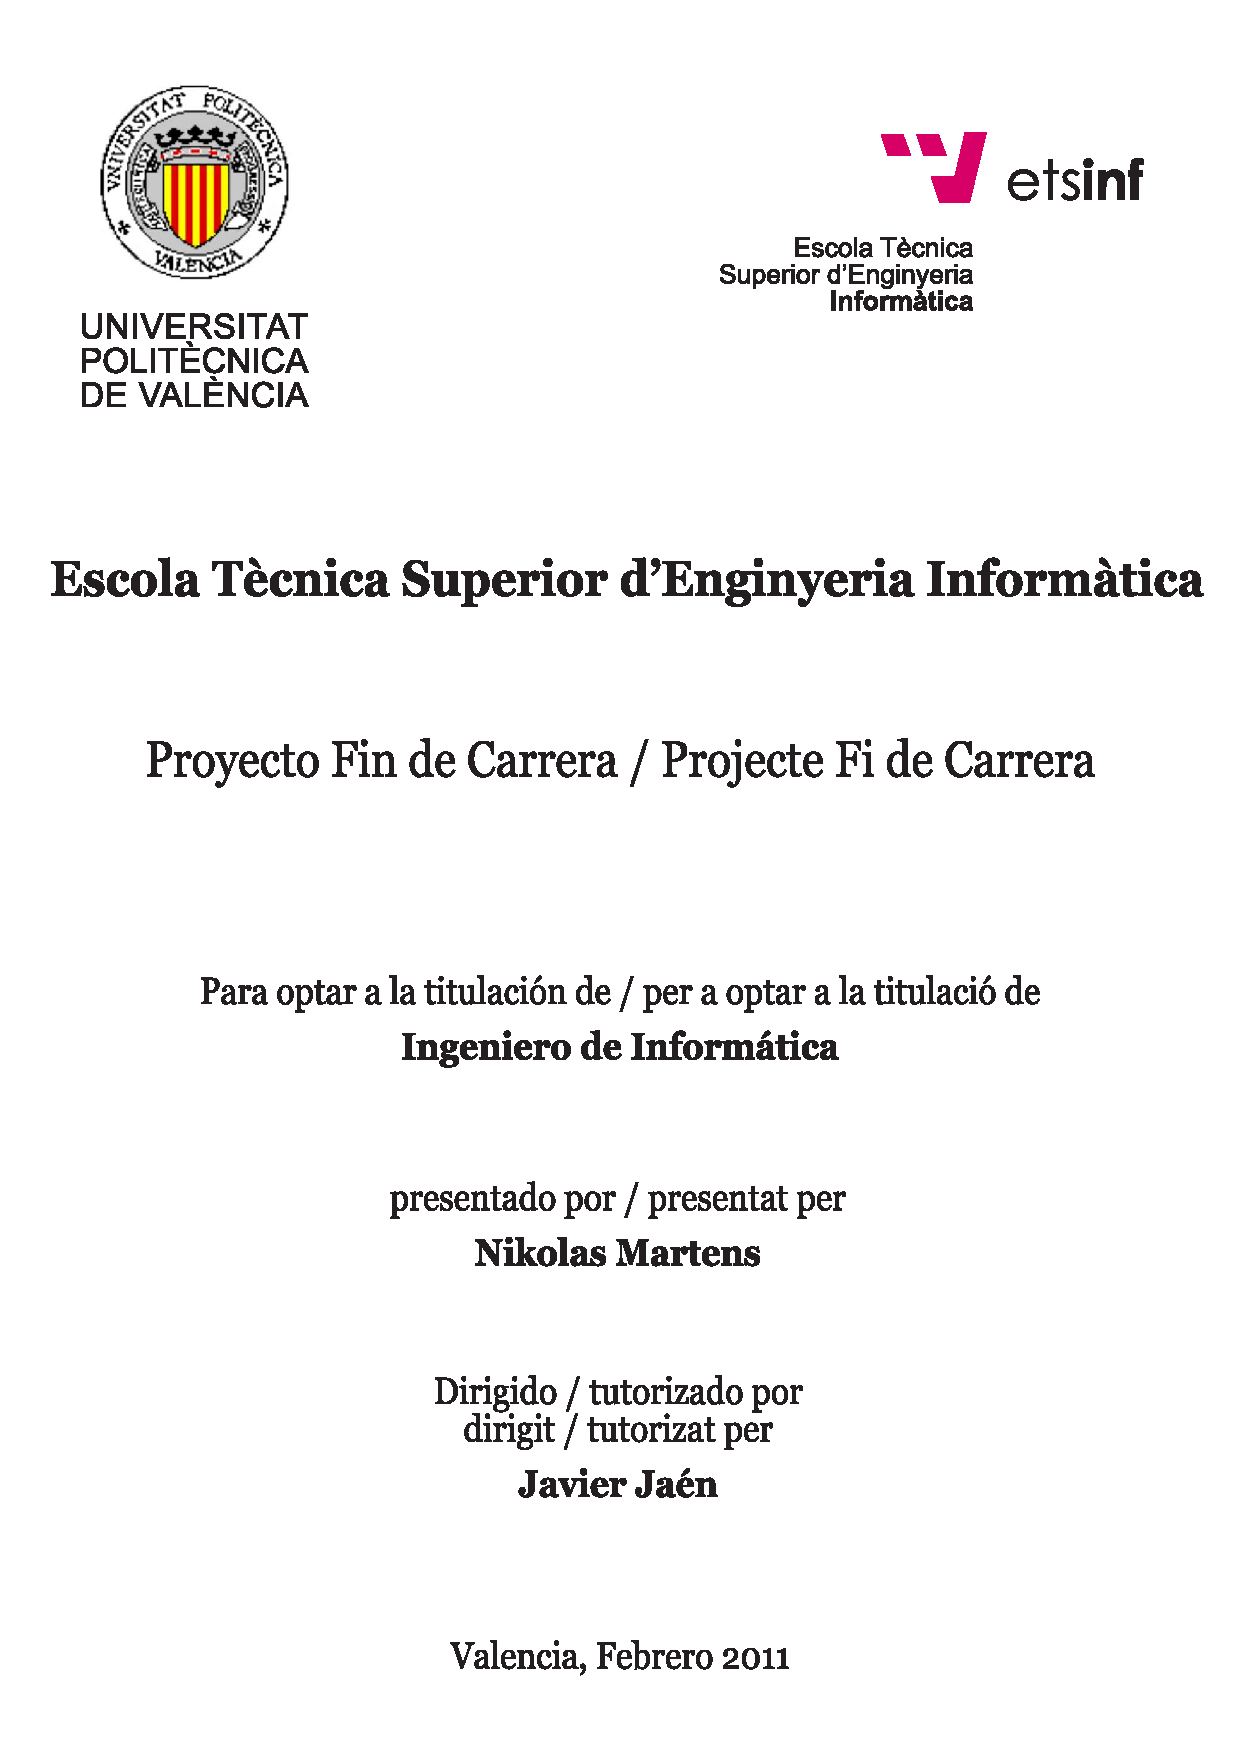
\includepdf{figures/portada}

%\newpage
%\thispagestyle{empty}
%\mbox{}

\maketitle  % command to print the title page with above variables


%: ----------------------- cover page back side ------------------------
% Your research institution may require reviewer names, etc.
% This cover back side is required by Dresden Med Fac; uncomment if needed.

%\newpage
%\vspace{10mm}
%1. Reviewer: Name
%
%\vspace{10mm}
%2. Reviewer: 
%
%\vspace{20mm}
%Day of the defense:
%
%\vspace{20mm}
%\hspace{70mm}Signature from head of PhD committee:
%


%: ----------------------- tie in front matter ------------------------

\frontmatter
%\include{0_frontmatter/dedication}
% Thesis Acknowledgements ------------------------------------------------


%\begin{acknowledgementslong} %uncommenting this line, gives a different acknowledgements heading
\begin{acknowledgements}      %this creates the heading for the acknowlegments

I would like to thank my advisor, Javier Jaén, for his valuable feedback and support in many ways during the projects and Prof. Klaus Diepold who gave me the opportunity to write this thesis. I also feel deepest gratitude to my friend Robert Jenke who gave me the idea and the courage to write about this topic. Lastly, I thank my family for their unconditional support.

\end{acknowledgements}
%\end{acknowledgmentslong}

% ------------------------------------------------------------------------





%: ----------------------- abstract ------------------------

% Your institution may have specific regulations if you need an abstract and where it is to be placed in the document. The default here is just after title.

\cleardoublepage 

% Thesis Abstract -----------------------------------------------------


%\begin{abstractslong}    %uncommenting this line, gives a different abstract heading
\begin{abstracts}        %this creates the heading for the abstract page

Although personal computing has advanced and spread considerably during the last decades, the real computer revolution has not happened yet. In order to promote computer literacy, a system is needed that enables the user to use the power of abstraction for building and arguing about dynamic models. This thesis presents a programming model that follows the paradigm "everything is an object" \cite{SmalltalkBlueBook} to the utmost in order to build a software platform upon it that provides this possibility. The result is a lean yet powerful model based on a single kind computational units which form a virtual network. All entities of the model are therefore concurrent, distributed and persistent. Like objects, they encapsulate behaviour and state and communicate through message passing, but unlike conventional objects, an entity has no methods, messages are asynchronous, the only structure is composition and the only association is specialization.

\end{abstracts}
%\end{abstractlongs}


% ---------------------------------------------------------------------- 

\markboth{}{}

% The original template provides and abstractseparate environment, if your institution requires them to be separate. I think it's easier to print the abstract from the complete thesis by restricting printing to the relevant page.
% \begin{abstractseparate}
%   
% Thesis Abstract -----------------------------------------------------


%\begin{abstractslong}    %uncommenting this line, gives a different abstract heading
\begin{abstracts}        %this creates the heading for the abstract page

Although personal computing has advanced and spread considerably during the last decades, the real computer revolution has not happened yet. In order to promote computer literacy, a system is needed that enables the user to use the power of abstraction for building and arguing about dynamic models. This thesis presents a programming model that follows the paradigm "everything is an object" \cite{SmalltalkBlueBook} to the utmost in order to build a software platform upon it that provides this possibility. The result is a lean yet powerful model based on a single kind computational units which form a virtual network. All entities of the model are therefore concurrent, distributed and persistent. Like objects, they encapsulate behaviour and state and communicate through message passing, but unlike conventional objects, an entity has no methods, messages are asynchronous, the only structure is composition and the only association is specialization.

\end{abstracts}
%\end{abstractlongs}


% ---------------------------------------------------------------------- 

% \end{abstractseparate}


%: ----------------------- contents ------------------------

\setcounter{secnumdepth}{2} % organisational level that receives a numbers
\setcounter{tocdepth}{2}    % print table of contents for level 3
\tableofcontents            % print the table of contents
% levels are: 0 - chapter, 1 - section, 2 - subsection, 3 - subsection

%: --------------------------------------------------------------
%:                  MAIN DOCUMENT SECTION
% --------------------------------------------------------------



% the main text starts here with the introduction, 1st chapter,...
\mainmatter

%\renewcommand{\chaptername}{} % uncomment to print only "1" not "Chapter 1"


%: ----------------------- subdocuments ------------------------

% Parts of the thesis are included below. Rename the files as required.
% But take care that the paths match. You can also change the order of appearance by moving the include commands.

\parskip = 2ex plus 1ex minus 1ex


% this file is called up by thesis.tex
% content in this file will be fed into the main document

%: ----------------------- introduction file header -----------------------

% the code below specifies where the figures are stored
\graphicspath{{figures/introduction/}}

% ----------------------------------------------------------------------
%: ----------------------- introduction content ----------------------- 
% ----------------------------------------------------------------------

\chapter{Introduction}
\label{chap:introduction}

Personal computing has made remarkable advances and became omnipresent during the last decades but like Turing Award winner and personal computing pioneer Alan Kay states repeatedly "the computer revolution has not happened yet" \cite{ComputerRevolution}. Computers have not yet had an impact comparable to the printing press for example, which not only changed completely how argumentation was done but also what was argued about. This change took approximately 150 years to happen so it is not a surprise that 30 years after their introduction, personal computers are still used as a faster and cheaper imitation of paper, recordings, films and television.

In order for a computer revolution to happen, \textit{computer literacy} needs to reach a critical mass, which is not only the ability to read and write but also to understand and argue about ideas that are worth writing about. What words are to printing, dynamic models are to computing, thus computer literacy is the ability to analyse and build models, understand the ideas they represent and use them to argue about these ideas.

This requires tools to build and share dynamic models like letters and books are used for printing. But in computer science still no common set of letters exists and the tools are only available to a small group of specialized users called programmers. Two of the most powerful tools are abstraction and distribution.

\section{Abstraction}

The single most important principle of computer science is abstraction \cite{ComputingDiscipline, abstractionInCs, StructureOfComputerPrograms}. It began with the division of software and hardware in the \textit{von Neumann} architecture and was continued with the appearance of programming languages and operating systems. With the increasing computational power, every generation of programming languages used a higher level of abstraction of the machine it is running on. 

Not only the abstraction of the programming models has evolved but also the ability to create new abstractions with the language \cite{Generations}. This development led from the first machine language over assembly languages to high level languages. At the cost of performance, each generation increased the expressiveness of the programming language and thus decreased the time necessary for development and maintenance. As a result, modern object-oriented languages do not require any knowledge of the underlying hardware and can be used efficiently to model dynamic software systems.

Besides the ability to build more complex systems in less time, abstraction also brings the advantages of re-usability and interoperability \cite{PowerOfAbstraction}. By hiding differences and emphasizing similarities, abstract models can be re-used for different but similar problems and communicate with each other more easily by ignoring unimportant details.

All of these advantages however, are restricted to the production of software. Because internals of a computer program are invisible to the end user, he can not benefit from the concepts used to build it. The world of the end user, which consists of files and programs has little connection with the world of objects, which resides inside programs. This affects software developers more than users since most programs work around this deficiency and hide it from the user. But few programs or software platforms let their users profit from the full power of abstraction. As a consequence, in personal computing there are many almost-the-same things which have to be treated differently because there exists no abstraction for them. An example are common problems with different file formats and encodings for documents, pictures and videos which require different viewers. Also web pages and local programs are nowadays quite similar but work differently for historical reasons.

It is also due to historical reasons that many modern programming languages lack of consistency \cite{ReshapingJava}. Some of the most widespread languages for example use a hybrid approach for backwards compatibility \cite{JavaCritics} and to allow access to lower abstraction levels \cite{CppCritics}. While different levels of abstraction are important to optimize efficiency, the lack of consistency increases the complexity of the programming models and compromises their expressiveness. These approaches also violate the core system building principle of separating meaning and optimization \cite{Steps2008}. But even the most purely object-oriented languages involve parts which are not objects or substantially different, such as packages, modules, methods or closures. Other components are not even part of the object model and can not be abstracted at all or only with difficulties such as location, file systems and databases.

\section{Distribution}

When the World Wide Web was designed for sharing scientific documents, its creators did not anticipate the way it was going to be used twenty years later. The strength and weakness of HTTP\nomenclature{HTTP}{Hypertext Transport Protocol} and HTML\nomenclature{HTML}{Hyptertext Mark-up Language} is simplicity and the resulting proliferation. Due to its limitations, a vast ecosystem of complement technologies has emerged to provide rich internet applications without compromising accessibility. Nowadays, even a simple dynamic web page involves at least four different technologies plus the knowledge of differences amongst interpreters.

Despite these hurdles, the popularity of internet applications has increased significantly over the last decade. This development has led to a browser-centric usage in personal computing today which resembles the use of terminal computers in the '80s. Internet applications run mostly on powerful servers with a very slim client which provides little more than a graphical interface for user interaction. For the software producers this brings many advantages in the areas of deployment, maintenance, scaling and not at last control over user data. The user does not only have to accept the lost of control over his data but also has do deal with conflicting software models which results in bookmarks and "back" buttons being mostly useless in internet applications.

A software platform which is aimed at the needs of modern personal computing would provide the the possibility to connect to any other system and share any kind of data in a safe and transparent way. To be able to do so, data must not be static but consist of dynamically responding entities that carry all information with them that is needed for presentation and manipulation. Also, these entities can be communicated with and their abilities explored dynamically. Using a common minimal interface for presentation and interaction, all parts of such a system could be used interchangeably when used to assemble new systems.

The biggest increase of productivity in software development does not come from more powerful tools or programming languages but from software reuse \cite{SilverBullet}. The majority of programming tasks consists of connecting existing software modules rather than creating new ones. But still, the wheel is re-invented many times since there is no wide-spread completely distributed system of dynamically explorable modules. Such a system would give every user access to a global collection of already existing solutions and also the ability to share his own ideas with the world.

It would also leverage the power of connection to create a \textit{personal internet} whose users are able to connect their own devices as peers to form a virtual computer whose data is distributed over the peers and only dynamically cached on the devices. This way any personal information and programs can be accessed in the same manner as any other resource made available by other users without compromising privacy but also without having to distinguish between local and remote services. There does not even exist a distinction between data and programs since all parts of the system are dynamic.

\section{Aims}

In order to build a completely coherent personal computing system that separates meaning from optimization, it has to be based on a programming model that incorporates the concepts of abstraction and distribution. It has to enable the user to dynamically model software systems inside a virtual space in a manner close to natural processes. This programming model has to be implemented into a runtime environment that supports the complete personal computer platform.

The result is a model of virtual objects which exist independent of any hardware. Computers only serve as portals that connect the virtual with the real world. Objects are living things that can be interacted with by sending them messages. To keep the communication as simple as possible, it is unidirectional, the receiver always reacts in the same way and the message is another object. Systems that are too complex to be modelled by a single object are composed by objects in \textit{has-a} relationships. And to allow abstraction, objects also have \textit{is-a} relationships with other objects.

The model is an abstraction of other object-oriented programming models, based on asynchronous message passing, prototypes and inheritance. It is an abstraction because it uses only one entity to encapsulate behaviour and state which plays the roles of classes, objects, methods and closures. Furthermore, it imposes a minimum of structure and protocol to increase interoperability and extensibility. It also can be arbitrarily nested and uses specialization and inheritance. The model is completely distributed which means it treats all objects equally, regardless of their location. As a consequence, it is also completely concurrent since all computation can possibly be carried out on different systems.

\section{Characteristics}

These requirements are fulfilled by the programming model presented in this thesis which has the following characteristics. To the best of our knowledge, no other software platform or programming language possesses all of these characteristics.

\begin{description}
\item[Completely concurrent.] Objects are independent of processor units and react instantly to a message. The only operation is therefore asynchronous message passing. The model includes a form of data flow for synchronization.

\item[Completely late bound.] Messages can only be sent to an object using its address. An address is always name-based thus all communication is late bound.

\item[Completely distributed.] Objects are also independent of physical memory so they are not bound to any device but are distributed in a network connecting an arbitrary number of devices. Name resolution is performed by the objects, leading to a distributed directory.

\item[Completely persistent.] Since objects do not depend on any hardware, they are not destroyed if a program is closed or a device shut down. Once created, an object continues existing until deleted explicitly.

\item[Completely dynamic.] All objects of the model can have behaviour, i.e. are dynamic and living entities. New objects are created and existing ones modified by sending messages to other objects. Hence there is no intrinsic distinction between compile and run time.

\item[Minimal structure.] Objects do not have any internal structure but can form compositional hierarchies. Thus objects serve as modules by containing other objects in a part-whole relationship. There are no classes, but objects serve as prototypes for new objects. Objects also do not have methods but always react with the same behaviour.

\item[Minimal association.] Except composition, the only association between objects is specialization. An object that specializes another object inherits all of its properties.

\end{description}

\section{Outline}

This thesis presents the implementation of the described programming model as the prototype of a software platform. Methods and techniques used during its development are described in the following chapter. 

The architecture of the resulting platform is illustrated in Figure \ref{fig:architecture} with the outline of the chapters describing its parts indicated by arrows. Chapter \ref{chap:programming_model} contains a detailed description of the programming model supported by a biological metaphor, an iterative example and the implementation of the platform's kernel. The kernel's environment is presented in Chapter \ref{chap:development_environment} consisting of mechanisms to connect the kernel to the local and remote systems and library support for reflection and generic components. Chapter \ref{chap:graphical_interface} describes graphical development tools on application level. 

The remaining chapters contain a discussion of results of the project and an outlook on future challenges along with conclusions.

\figuremacro{architecture}{Architecture of software platform}
{Architecture of the software platform and outline of this document.}


\graphicspath{{figures/methods/}}

%: ----------------------- name of chapter  -------------------------
\chapter{Methods}

This chapter describes the methods and techniques used during the development of the presented software platform. Due to the explorative nature of the project, methods supporting an iterative style of development were chosen. The following sections describe different approaches to software engineering and two applied methods in more detail.

%: ----------------------- section ------------------------
\section{Software Development}

According to the IEEE\nomenclature{IEEE}{Institute of Electrical and Electronics Engineers}, software development is part of software engineering which is defined as (1) The application of a systematic, disciplined, quantifiable approach to the development, operation, and maintenance of software; that is, the application of engineering to software. (2) The study of approaches as in (1). \cite{IeeeGlossary}

There are generally two classes of methodologies, independent of their field of application. The \textit{top-down} method starts with the abstract and proceeds to the concrete while the \textit{bottom-up} follows the opposite direction. \cite{Balzert}. In software development, the two classes correspond to the general fields of \textit{structured} methods and \textit{agile} approaches, respectively. While structured methods focus on predictability, agile development puts more emphasis on adaptation.

The NATO\nomenclature{NATO}{North Atlantic Treaty Organization} Software Engineering Conference in 1968 \cite{NatoConference} marks the beginning of systematic approaches to software development in order to address issues caused by the complexity of computer programs \cite{HumbleProgrammer}. Early manifestations of this approach are the waterfall model and structured programming. As illustrated in Figure \ref{fig:waterfall_model}, the former models the development process as a linear sequence of several phases, with the output of each phase being the input of the next. While its strict linearity was already described by its introducer as being risky and inviting failure \cite{ManagingLargeSystems}, the model has reached widespread acceptance and popularity.

\figuremacro{waterfall_model}{Waterfall model with six phases}
{A waterfall process model with six phases: Requirements, Analysis, Design, Coding, Testing and Operation.}

The waterfall process model is an extreme on the continuum between top-down and bottom-up methods and is only applicable for solutions to very well understood problems which can be completely planned and designed in advance. Since in practice this type of project is very rare, modified waterfall models have been introduced which allow iteration by providing feedback channels between certain or all phases.

Agile software development is placed on the other end of the continuum and recommends many iteration of the complete process in very short cycles in the magnitude of weeks. It uses process models such as the spiral model which adds the dimension of \textit{completeness}. Figure \ref{fig:agile_model} illustrates the transition from a iterative waterfall model to the spiral model. According to this model, the development runs through all phases with only a small subset of the product's requirements and increases the set with each iteration.

\figuremacro{agile_model}{Transition from waterfall to spiral model}
{Transistion from linear waterfall model to iterative spiral model using feedback channels.}

Although used in practice as early as the 1950s, public awareness of agile development methods was very low until the 1990s when most standardized method emerged such as Scrum, Feature Driven Development (FDD\nomenclature{FDD}{Feature Driven Development}) and Extreme Programming (XP\nomenclature{XP}{Extreme Programming}) \cite{AgileHistory}. These methods gained very quickly popularity especially in the development of internet applications. The term \textit{agile development} was introduced in 2001 by the \textit{Manifesto for Agile Software Development} \cite{AgileManifesto}.

In practice, software projects use a methodology located between these two extremes, considering project and team size, budget, time limits and other influences. More stable and well understood projects use fewer and longer iteration cycles while more risky and dynamic projects are best suited with shorter cycles and releasing often.


%: ----------------------- section ------------------------
\section{Prototyping}
\label{sec:prototyping}

Due to its explorative nature, an agile software development method was used in this project called \textit{rapid prototyping}. A prototype is a executable program which does not implement all features required for the final product but only those that serve a specific purpose. The method follows the spiral model illustrated in Figure \ref{fig:agile_model} where each iteration produces a prototype which is used for experiments to revise existing requirements and determine new ones.

The advantage of prototyping is a tight feedback loop. Errors in analysis and design are identified early while the cost of changes is still low. Prototypes are also a useful mean to facilitate communication with a client or amongst developers since concrete implementations can be discussed instead of abstract descriptions. Disadvantages of prototyping are increased costs during early stages of a project and the risk of distraction from proper analysis which may lead to a decreased robustness. These characteristics also hold true for other iterative development methods. The unique character of prototyping is that it prototypes do not necessarily form the base of future iteration but are often thrown away.

During this project, prototyping was used to verify and improve the programming model. The model was implemented with low cost into a prototype which was then used to verify the model using experiments. Several level of experiments were used reaching from simple message passing in different cell system constellations to complete example applications. Each prototype lead to an improved version of the programming model or the binding algorithm which was implemented into a new prototype. In total, eight iterations were traversed during the project.


%: ----------------------- section ------------------------
\section{Test-Driven Development}
\label{sec:tdd}

A technique tightly coupled with agile software development is \textit{Test-Driven Development} (TDD\nomenclature{TDD}{Test Driven Development}). As shown in Figure \ref{fig:tdd}, the testing and development phases of the waterfall model are swapped, putting testing first. The model is best suited for the development of small, independent functional units which can be validated by automated tests called \textit{unit tests}. This proceeding has several advantages: \cite{TestDrivenDevelopment}

\begin{description}
\item[Better tests.]{Programmers tend to avoid critical constellations -- mostly unconsciously -- if they exactly know what the tested code is doing. Tests written beforehand are less prejudiced.}

\item[Better design.]{When writing a test first, the developer has to think about a module's interface before its implementation. Writing small, clearly structured and loosely coupled modules is enforced since convoluted systems are not testable. If a module cannot be tested, it is refactored.}

\item[Confidence.]{Being able to test each part of a system at any time, project members
become more confident about its reliability. Refactoring becomes less dangerous
and is performed more often \cite{FowlerRefactoring}.}

\item[Higher test coverage.]{Writing tests is a tedious task and mostly not done because
of time pressure. Doing it first requires less discipline and results in more tests.}

\end{description}

\figuremacro{tdd}{Process model of test-driven development}
{Process model of test-driven development.}

The applicability of TDD is limited by the range of automated testing. Concurrent processes, graphical user interfaces and system integration can not or only with difficulty be tested automatically \cite{ExtremeProgramming}. In some cases the method can still be applied by designing tests which require manual validation before implementation.

In this project, TDD was applied with great success to implement all of the described parts of the software platform. The characteristics of automated testing as executable requirements specification proved especially useful with each new prototype. While the design of the system changed significantly between two iterations, the test suite almost did not changed and thus ensured that the new prototype provides all features of the last one including all bug fixes. In average, each prototype used approximately 70 unit tests.

Test-Driven Development is to a development cycle like the development cycle to the project. It provides a tight feedback loop and enables the developer to solve a problem in small steps. Like development cycles, the size of the steps can be adapted to the problem. Big steps can be taken on well known ground and small steps on new ground or when a big steps fails.


\graphicspath{{figures/programming_model/}}

\chapter{Programming Model}
\label{chap:programming_model}

This chapter describes the programming model in a top-down fashion. The first section describes the concepts and design of the model, followed by the demonstration of these with the help of an example. The last section describes the implementation of the model. It covers only the parts which directly derive from the model, further parts of the kernel are described in Chapter \ref{chap:development_environment}.

%-----------------------------------------------------
%-----------------------------------------------------
\section{Concepts}
\label{sec:concepts}

The programming model is presented in this section by introducing its concepts individually using the metaphor of a biological cell as suggested in \cite{SmalltalkHistory}.

%-----------------------------------------------------
\subsection{Cells}

The model consists of a single kind of behavioural building block called \textit{cell}. Like biological cells, these virtual cells live independent of each other and are able to react concurrently. Cells can be nested arbitrarily. Nested cells are called \textit{children} and the containing cell \textit{parent}. This results in a hierarchical structure with a global \textit{root} cell named "$\circ$". Figure \ref{fig:cells} illustrates nested cells.

\figuremacro{cells}{Nested cells}
{A single kind of hierarchically structured behavioural building block.}

%-----------------------------------------------------
\subsection{Names and Paths}

Each cell has a name which is unique amongst its siblings. A parent cell can address one of its children using its name. Children can address their parent cell using "parent" and the root cell with "$\circ$". A cell can always address itself using "self". Cell names can be combined to form a cell \textit{path} which leads from an origin to a destination cell. Cell paths are analogue to paths in file systems where ".", ".." and "/" correspond with "self", "parent" and "$\circ$" respectively. These references are called \textit{aliases}.

Figure \ref{fig:names} illustrate an example of nested cells with names and aliases. In this example, the path \cell{Roots.parent.Trunk.Branch} (using dots to separate cells) leads from \cell{Tree} to \cell{Branch}. 

\figuremacro{names}{Nested cells with names and aliases}
{Nested cells with names and aliases.}

%-----------------------------------------------------
\subsection{Messages}

The only way of communication between two cells is by sending messages. A message is a cell which is sent from a sender to a receiver cell as illustrated in Figure \ref{fig:message}. Message passing is always asynchronous which means that the sender does not wait for the message to be received and processed.

\figuremacro{message}{Message passing}
{A message is being sent from a sender to a receiver cell.}

%-----------------------------------------------------
\subsection{Reaction}
\label{sec:reaction}

A cell reacts on the event of receiving a message. All cells contain a description of how to react called \textit{reaction} which is executed each time the cell receives a message. As shown in Figure \ref{fig:reaction}, a reaction consists of \textit{mailings}, each containing the paths of the receiver and message cell, both relative to the sender. During execution, each mailing of the reaction is processed simultaneously, i.e. each message is sent to its corresponding receiver cell.

\figuremacro{reaction}{Reaction of a cell}
{A cell with its reaction consisting of mailings.}

%-----------------------------------------------------
\subsection{Specialisation}

As with biological cells, the only way to create a new cell is by \textit{specializing} an existing cell. The created \textit{sub-cell} inherits all properties of the \textit{stem} cell which includes children and reaction. As depicted in Figure \ref{fig:specialisation}, the sub-cell can add further children or replace an inherited child or reaction, but it can not remove an inherited child. The relationship is strictly unidirectional and dynamic. This means that no change of the sub-cell can affect the stem cell but changes to the stem cell affect all sub-cells instantly. Also, the stem cell of an existing cell can be changed.

\figuremacro{specialisation}{Example of specialisation}
{\cell{John} specializes \cell{Person}, inherits \cell{Hands}, replaces \cell{Eyes} and extends it with \cell{Glasses}.}

%-----------------------------------------------------
\subsection{Execution}
\label{sec:execution}

The reaction is not executed by the receiver cell directly but by a new child which specializes the receiver. This \textit{execution cell} extends the receiver by the alias \cell{message} which is connected with the message cell as shown in Figure \ref{fig:execution}. Aliases can be compared with hard links in file systems thus \cell{X.message.parent} does not resolve to \cell{X} but to the parent of \cell{M}. The execution cell can also be extended by further children and therefore provide a storage space for local results which only matter to the execution.

\figuremacro{execution}{Creation of execution when receiving a message}
{A receiver creates a new execution that executes the reaction and which extends the receiver with an alias to the message cell.}

%-----------------------------------------------------
\subsection{Delivery}
\label{sec:delivery}

A message might not be delivered because of three possible reasons: an error, a non-existent receiver or a deactivated receiver. In either case, the message is re-sent until delivered successfully or explicitly cancelled. This enables messages to be sent to cells before they exist, e.g. results before they are calculated, which can be used for data flow synchronization as illustrated in Figure \ref{fig:data_flow}. A deactivated cell can not receive any message and deactivates all children except those that give access to its internal properties such as stem, reaction and children. This way cells with incomplete definitions can be made inaccessible.

\figuremacro{data_flow}{Data flow synchronization}
{Data flow synchronization of the the calculation $3 \cdot 4 + 2 \cdot 3$. The summation is executed earlier but waits for both multiplications.}

%-----------------------------------------------------
%-----------------------------------------------------
\section{Example}
\label{sec:example}

The presented concepts of the programming model are illustrated in this section using an example application. The example is divided into two versions. A simple version illustrates the most basic concepts and an extended version illustrates the remaining concepts.

Cells are defined in tables containing the hierarchy, name, stem cell path and reaction of the cell. Paths are written using dots to separate parents and children where \cell{parent} references are abbreviated with $\rho$. The mailings of reactions are written as "$receiver \leftarrow message$" where $receiver$ and $message$ are paths relative to the defined cell. Instead of using mailings, reactions may be described informally or left undefined and therefore inherited by the stem cell.

%-----------------------------------------------------
\subsection{Simple Version}

The example application is a simple publish-subscribe system. Several cells can \textit{subscribe} to a channel and, as a result, receive all messages that have been \textit{published} on that channel. 

\subsubsection{Definition}

Table \ref{tab:simple_example} contains the definitions of the involved cells. Top-level cells are children of the root cell.

\tablemacro{simple_example}{lll}{Cell definitions of simple example application}
{Cell definitions of simple publish-subscribe example application.}
{\bf{Cell}                    & \bf{Stem} & \bf{Reaction}}
{Channel                      & Cell      & $subscribers.each \leftarrow forwardMessage$\\
\texttt{|\_} forwardMessage   & Cell      & $message \leftarrow \parent.\parent.message$\\
\texttt{|\_} subscribers      & List\\

\hline

Cell                          & Cell      & Does nothing\\
List                          & Cell\\
\texttt{|\_} each             & Cell      & Sends each element to its \cell{message}\\
\texttt{|\_} add              & Cell      & Creates new element with message as stem\\}

The first three rows define cells specific to the publish-subscribe application. The following definitions are generic cells which are part of a standard library and included for completeness. The specific cells are \cell{Channel} with its two children \cell{forwardMessage} and \cell{subscribers}. The cell \cell{Cell} is the default stem cell and the root of all specialisation hierarchies. Figure \ref{fig:simple_example} illustrates the defined cells and their relationships.

\figuremacro{simple_example}{Defined cells for simple example application}
{Composition (a) and inheritance (b) hierarchies of defined cells for a simple publish-subscribe system.}

A cell can be published on the \cell{Channel} by being sent to it as a message. Every time the \cell{Channel} receives a message, its reaction is executed, i.e. its child \cell{forwardMessage} is sent to the child named \cell{each} of \cell{Channel}'s child \cell{subscribers}. Note that \cell{subscribers} inherits \cell{each} from \cell{List}. The reaction of \cell{each} is implemented on the kernel level and sends each of the list's elements to the cell that was received by \cell{each}, in this case \cell{forwardMessage}.

As a result, \cell{forwardMessage} receives each of \cell{subscribers} elements. The instruction of \cell{forwardMessage}'s reaction is then executed with each subscriber as its \cell{message} and sends the published cell (the message received by \cell{Channel}) to each subscriber (message sent to \cell{forwardMessage} by \cell{subscribers.each}).

\subsubsection{Execution}

The two \cell{parent} references (abbreviated with $\rho$) in the reaction of \cell{forwardMessage} are necessary because the reaction does not execute in the context of the receiver cell but in the context of its execution cell as described in Section \ref{sec:execution}. If cells play the role of methods, executions play the role of their activation records. Unlike activation records, executions do not cease to exist when the reaction completes since executions are accessible from within other executions and due to the asynchronism of message passing they do not become unreachable.

The execution cell is a specialisation of the receiver cell, therefore inherits all of its children and can send them messages as done in the reaction of \cell{Channel}. Thus the first \cell{parent} of \cell{forwardMessage}'s reaction references the \cell{forwardMessage} cell and the second \cell{parent} references the execution of \cell{Channel}'s reaction.

Figure \ref{fig:execution_example} illustrates executions and \cell{message} aliases with a subset of the cells involved in the example application. Executions are depicted as name-less cells which are children and sub-cells of the receiver cell and have a \cell{message} alias as child. In the example, \cell{each} sends a message to its \cell{message} child (see Table \ref{tab:simple_example}) but because of the alias, the message is received by \cell{forwardMessage} (labelled "fm" in the figure). Because the reaction of \cell{forwardMessage} runs within its execution, the channel's message is the \cell{message} child of its execution which is two parents up from \cell{forwardMessage}'s execution.

\figuremacro{execution_example}{Execution cells in the example application}
{Mailings and resulting execution cells of the simple publish-subscribe system. \textbf{(a)} A publisher sends a message to \cell{Channel} which creates an \textit{execution} with a \cell{message} alias as child. \textbf{(b)} Eventually \cell{forwardMessage} (fm) receives a subscriber as message and creates an execution as well. \textbf{(c)} The execution is a child of \cell{forwardMessage} so the published cell is its parent's parent's message.}

\subsubsection{Usage}

To actually use the system, subscriber cells have to be added to the channel and cells be published. Table \ref{tab:simple_example_usage} contains the definitions of subscribers and the driver cells \cell{Initialize} and \cell{Run}, whose reactions add subscribers to a channel and publish a literal string on it.

\tablemacro{simple_example_usage}{lll}{Usage of simple example application}
{Definition of subscribers and driver cells to run the publish-subscribe example.}
{\bf{Cell}    & \bf{Stem} & \bf{Reaction}}
{subscriber1  & Cell    & Does something with its message\\
subscriber2   & Cell    & Does something with its message\\

\hline

Initialize    & Cell    & $\circ.Channel.subscribers.add \leftarrow \circ.subscriber1$\\
              &         & $\circ.Channel.subscribers.add \leftarrow \circ.subscriber2$\\
Run           & Cell    & $\circ.Channel \leftarrow \circ.Literal.String."Hello World"$\\}

%-----------------------------------------------------
\subsection{Extended Version}
\label{sec:example_extended}

In this section new features are added to the publish-subscribe system of the previous section to illustrate further concepts of the software platform. In the extended version of the application, a subscriber cell can influence whether it receives a published cell or not. This is done by adding subscriptions to a channel which contain logic to decide for each published cell whether its subscriber is interested in it or not. When a new cell is published, the channel sends it first to each subscription and only forwards it to the subscriber if the subscription replies positively.

\subsubsection{Responses}

Because message passing is asynchronous, a sender that expects a response has to send a cell along with the message that the receiver can respond to. This is done by creating a \textit{container} cell which specializes the actual message. By convention, the cell that the response is expected to be sent to is a child of the container named \cell{respond}.

Figure \ref{fig:responses} compares mailings (a) without and (b) with response. In the first case, \cell{A} sends \cell{M} to \cell{B} which cannot send any message as response since it has no information about \cell{A}. It could send a response to \cell{M} but if the same cell is sent more than once a correlation between messages and responses would be impossible. For this reason, \cell{A} sends a unique container cell \cell{C} (letter I in Figure \ref{fig:responses} (b)) which specializes \cell{M} and contains a cell \cell{R}, to which \cell{B} sends its response message (letter II).

\figuremacro{responses}{Mailing without and with response}
{Cells involved in mailing (a) without and (b) with response.}

\subsubsection{Definition}

The involved cells are defined in Table \ref{tab:extended_example}, which also contains the definitions of further library cells needed by the example. These definitions are complementary to previous definitions.

\tablemacro{extended_example}{lll}{Cell definition of extended example}
{Cell definitions of extended publish-subscribe example application.}
{\bf{Cell}                    & \bf{Stem} & \bf{Reaction}}
{Channel                      & Cell & $subscribers.each \leftarrow forwardMessage$\\
\texttt{|}                    &      & $subscriptions.each \leftarrow askSubscription$\\
\texttt{|\_} subscriptions    & List \\
\texttt{|\_} askSubscription  & Cell & $cell.create.wants \leftarrow \parent.\parent.message$\\
\texttt{  |}                  &      & $message \leftarrow wants$\\
\texttt{  |}                  &      & $wants.response.ifTrue \leftarrow forwardMessage$\\
\texttt{  |\_} forwardMessage & Cell & $\parent.\parent.message.subscriber \leftarrow \parent.\parent.\parent.message$\\
Subscription                  & Cell & $message.respond \leftarrow \circ.True$\\

\hline

Cell                          & Cell\\
\texttt{|\_} respond          & Cell & $\parent.\parent.cell.create.response \leftarrow message$\\
True                          & Cell \\
\texttt{|\_} ifTrue           & Cell & $message \leftarrow \circ$\\
False                         & Cell \\
\texttt{|\_} ifTrue           & Cell & does nothing\\}

The first definition extends the reaction of \cell{Channel} by a second instruction which iterates through the \cell{subscriptions} list (second definition) by sending the channel's child \cell{askSubscription} to its child \cell{each}.

The third definition contains the reaction of \cell{askSubscription} to which all the subscriptions of the channel are sent individually as messages by \cell{each}. The first instruction creates a new cell named \cell{wants} with the published cell (\cell{message} of the channel) as its stem. The new child is sent to the received subscription in the second instruction.

The new cell is created using \cell{cell.create} which is implemented on the kernel level and has an infinite number of children that create cells with their own name and the received message as stem. Note that \cell{wants} is created as a child of the execution cell and not of \cell{askSubscription}. In this case, the execution serves as a local name-space just like activation records. This way executions created by further subscriptions sent to \cell{askSubscription} are able to create their own \cell{wants} children without conflicting with other executions.

The child \cell{wants} plays the role of the before mentioned container cell which is necessary because it contains \cell{respond} (inherited by \cell{Cell}) which will receive the response. The reaction of \cell{respond} creates a cell named \cell{response} in the receiver's parent with the received cell as its stem.

This behaviour is used by a feature of the programming model called \textit{data flow synchronization} which is described in Section \ref{sec:delivery}. The third instruction of \cell{askSubscription}'s reaction sends a message to a child of \cell{wants.response}. This cell does not exist before \cell{wants.respond} has received a message. The instruction can still be executed because in the case of a non-existent receiver, a mailing is repeated until its message is delivered. This enables instructions to be processed before all of their required information is available.

The same instruction is also an example of library-based control structures. The reaction of \cell{forwardMessage} is only executed if the response is a sub-cell of \cell{True} since only \cell{True} defines a reaction for its \cell{ifTrue} child.

The last definition for the system is a prototype of \cell{Subscription} which provides a default reaction by responding with \cell{$\circ$.True}.

\subsubsection{Usage}

As in the previous section, driver cells are needed in order to run the application. The cells defined in Table \ref{tab:extended_example_usage} create two channels by specializing \cell{Channel} and two subscriptions for \cell{subscriber1} of the previous example. The first subscription inherits the default reaction from its stem cell \cell{Subscription} and the second subscription executes its stem cell's reaction explicitly by forwarding its \cell{message} to its child \cell{stem} which works like \textit{super} in conventional object-oriented languages. And as before, cells are defined to initialize and run the example.

\tablemacro{extended_example_usage}{lll}{Usage of extended example application}
{Definition of channels, subscribers and driver cells to run the extended publish-subscribe example.}
{\bf{Cell}               & \bf{Stem} & \bf{Reaction}}
{channel1                & Channel      \\
channel2                 & Channel      \\
subscription1            & Subscription \\
\texttt{|\_} subscriber  & subscriber1  \\
subscription2            & Subscription & $\parent.stem \leftarrow message$\\
\texttt{|\_} subscriber  & subscriber1  \\
\hline
Initialize               & Cell         & $\circ.channel1.subscriptions.add \leftarrow \circ.subscription1$\\
                         &              & $\circ.channel2.subscriptions.add \leftarrow \circ.subscription2$\\
Run                      & Cell         & $\circ.channel1 \leftarrow \circ.Literal.String."Hello World"$\\
                         &              & $\circ.channel2 \leftarrow \circ.Literal.String."Hello World"$}

%-----------------------------------------------------
%-----------------------------------------------------
\section{Implementation}
\label{sec:implementation}

This section describes the implementation of the object model, how mailings are processed, cell paths bound to executions and other functional parts that derive directly from the programming model. Parts of the implementation regarding the environment of the software platform such as storage, distribution, reflection and libraries are described in the next chapter.

%-----------------------------------------------------
\subsection{Object Model}

The class diagram in Figure \ref{fig:class_diagram} shows the classes and their associations used to implement the object model described in Section \ref{sec:concepts}. Each class is described roughly in the following list and their functionality in the following sections.

\figuremacro{class_diagram}{Class diagram of object model}{Class diagram of object model.}

\begin{description}
\item[Cell]{Implements compositional cell hierarchies with each instance referencing its parent and children objects. The tree may be incomplete since children are loaded on-demand but an upwards branch is always completely loaded.}

\item[Deliverer]{Interface for classes that are able to deliver a message such as \code{Cell} and \code{Peer}. The latter is described in Section \ref{sec:distribution}.}

\item[Reaction]{Implements the reaction of the programming model which executes a list of mailings.}

\item[NativeReaction]{An abstract type for reactions that may execute any kind of code. Being able to perform computations without sending messages, subclasses of this class break the otherwise endless recursion of message passing.}

\item[Mailing]{Stores paths of receiver and message cells.}

\item[Path]{Represents a cell path as a list of strings, each string being a cell name.}

\item[Messenger]{Every mailing is delivered by its own messenger instance which spawns a new thread an re-tries sending its message until the delivery returns a positive result.}

\item[Delivery]{Holds parameters which are stacked for nesting deliveries (see Section \ref{sec:inheritance}).}

\item[DeliveryId]{Unique identifier to avoid circular deliveries.}

\item[Result]{Return value of deliveries to determine success and return logged information.}

\item[Execution]{Class of execution cell objects which is created for every received message. Contains local cells and resolves references to its message alias.}

\end{description}

%-----------------------------------------------------
\subsection{Message Passing}

The reaction of a cell is executed each time the cell receives a message. This is done by invoking the method \code{execute()} which is declared by \code{NativeReaction} and implemented by \code{Reaction}. Listing \ref{lst:reaction_execute} shows the pseudo-code description of the implementation. 

The method processes a list of mailings. First, the \textit{role} of the execution is inserted at the beginning of the receiver and message paths. The role is the path of a cell as resolved during binding. It may differ from a cell's actual path due to inheritance as illustrated in Section \ref{sec:inheritance}. Thus by inserting the role at the beginning of the relative path, it is made absolute. A message is sent using a new instance of \code{Messenger}.

\begin{lstlisting}[mathescape, float=hbt, label=lst:reaction_execute, 
caption=Execute method of Reaction]
void execute (receiver, role, message, id) { {
	foreach (mailing in mailings) {
		mailing.receiver.insert(0, role);
		mailing.message.insert(0, role);
		
		new Messenger(receiver, mailing, role, id).start();
	}
}
\end{lstlisting}

The class \code{Messenger} spawns a new thread when instantiated in which the message will be re-sent until it is delivered successfully. This is done by the method \code{run()} of \code{Messenger} which is described in Listing \ref{lst:messenger_run}. In this method, a new delivery stack is created with a single delivery containing the role of the execution and the receiver path. A unique delivery identifier is created which is used to detect and avoid endless delivery loops. The resolution of the receiver cell is started by invoking the \code{deliver()} method of the sender cell.

\begin{lstlisting}[mathescape, float=hbt, label=lst:messenger_run, 
caption=Run method of Messenger]
void run() {
	do {
		if (!pausedAll) {
			var deliveryStack := new DeliveryStack();
			deliveryStack.add(new Delivery(role, mailing.receiver));

			var uid := new ExecutionId(eid, sender.count);
			sender.count := sender.count + 1;

			result := sender.deliver(deliveryStack, mailing.message, uid);
		}
	} while (!result.wasDelivered());
}
\end{lstlisting}


%-----------------------------------------------------
\subsection{Binding}
\label{sec:binding}

All references, even those to stem cells and enclosing cells, are late bound. The object model provides the structure for binding the path of a receiver cell to a reaction. This is done recursively by the method \code{deliver()}, defined in the \code{Cell} class. Each invocation of the method resolves a child of the current cell which may be inherited or located on remote sites. Listing \ref{lst:binding_algorithm} contains a pseudo-code description of the \code{deliver()} method.

\begin{lstlisting}[mathescape, float=htbp, label=lst:binding_algorithm, 
caption=Binding algorithm]
Result deliver (deliveryStack, message, id) {
	deliveryStack.popCompletedDeliveries();

	var delivery := deliveryStack.first;
	var nextCell := nil;

	if (searchedBefore(id, delivery.receiver)) 
		return new Result();

	if (delivery.receiver.isEmpty()) {
		if (reaction $\neq$ nil) {
			executeReacion(message, id, delivery);
			return new Result().deliveredTo(delivery.role);
		}
	} else {
		nextCell := getNextDeliverer(deliveryStack);
	}

	if (nextCell = nil) {
		addToSearchedBefore(id, delivery.receiver);
		var peerResult := tryPeers(deliveryStack, message, id);
		if (peerResult.wasDelivered())
			return peerResult;
	}

	var inherited := false;
	if (nextCell = nil and stem $\neq$ nil) {
		inherited := true;
		nextCell := this;
		deliveryStack.push(new Delivery(delivery.role, stem));
	}

	if (nextCell $\neq$ nil) {
		var nextResult := nextCell.deliver(deliveryStack, message, id);
		if (nextResult.wasDelivered()) {
			if (inherited 
					and nextResult.deliveredTo.contains(getPath())) {
				adopt(inheritedPath(nextResult), message, id);
			}
			return nextResult;
		}
	}

	return new Result();
}
\end{lstlisting}

The binding of a receiver path to a reaction begins with the sender cell which is the original receiver. The instance of \code{Messenger} processing the mailing passes the created \code{deliveryStack}, the path of the \code{message} cell and a unique execution identifier (\code{id}) to the \code{delivery()} method of the sender cell object.

The method starts with popping deliveries that have reached their receiver off the stack as explained in more detail in Section \ref{sec:inheritance}. The execution identifier is used in line 7 to avoid endless delivery loops caused by circular structures of stem cells or distributed cells. If a certain receiver was resolved by the same cell in the same delivery before, the resolution step fails by returning an empty \code{Result}.

Lines 10 and 11 check whether the current cell is the receiver and also contains a reaction. If so, the cell's reaction is executed by the auxiliary method \code{executeReaction()} which is described in Section \ref{sec:binding_execution}.

If the current cell is not the receiver, the next cell in the receiver path has to be found. This is done locally in line 16 using \code{getNextDeliverer()}. The method first checks if the next reference is an alias and resolves it as described in Section \ref{sec:aliases}. If it is not an alias, the child is searched for in the list of the cell's own children and returned.

If no next deliverer was found this way, the cell cannot resolve it locally and the delivery is forwarded to distributed parts of the cell by the method \code{tryPeers()}. The method and other details of distribution are described in Section \ref{sec:distribution}. If the receiver was found on a remote system, the delivery returns the positive result in line 23.

Otherwise, line 27 checks whether a next deliverer was found previously. If not, and a stem cell path is defined, the child or reaction is inherited by forwarding the delivery to the stem cell. This is done by pushing a new delivery to the stack as described in Section \ref{sec:inheritance}.

In line 33 the delivery is continued with the next deliverer that was found suitable during the algorithm and a possibly modified delivery stack. If the receiver was successfully inherited and is a child of the current cell, it is adopted in line 38 which is described in Section \ref{sec:adoption}. If no next deliverer was found, nor can the receiver be inherited because no stem cell path is defined, the delivery fails in line 44.

%-----------------------------------------------------
\subsection{Execution}
\label{sec:binding_execution}

As described in Section \ref{sec:execution}, the receiver cell does not execute the reaction itself but creates a child cell to do so. This is done by the method \code{executeReaction()} which is invoked in line 12 of Listing \ref{lst:binding_algorithm}. The pseudo-code description of the method is shown in Listing \ref{lst:reaction_execution} . 

\begin{lstlisting}[mathescape, float=htb, label=lst:reaction_execution, 
caption=Execution of reaction]
void executeReaction (message, id, delivery) (
	var executionName := "#" + id;
	if (delivery.role = getPath()) {
		addChild(new Execution(this, executionName, message));
	}
	delivery.role.add(executionName);

	reaction.execute(this, delivery.role, message, id);
}
\end{lstlisting}

The execution cell is created as a child of the receiver with a unique name composed of the delivery identifier. If the current cell was inherited (role does not equal path), the execution is not added and has to be adopted by the inheriting cell which is described in Section \ref{sec:adoption}. The stem cell path of the execution cell is set to \cell{parent} by its constructor. In the last line, the cell's reaction is executed under the context of the execution cell.

The \cell{message} alias of the execution cell is resolved by \code{Execution} by overriding the \code{getNext\-Deliverer()} method as shown in Listing \ref{lst:message_resolution}. The method checks if the next cell to be resolved has the name "message" and if so, removes it from the receiver path and inserts the message cell path instead.

\begin{lstlisting}[mathescape, float=htb, label=lst:message_resolution, 
caption=Resolution of message alias]
Cell getNextDeliverer(deliveryStack) {
	var delivery = deliveryStack.first;
	var name := delivery.receiver.first;

	if (name = "message") {
		delivery.receiver.removeFirst();
		delivery.receiver.insert(0, message);
		return this;
	} else {
		return super.getNextDeliverer(deliveryStack);
	}
}
\end{lstlisting}

%-----------------------------------------------------
\subsection{Aliases}
\label{sec:aliases}

In line 16 of the \code{deliver()} method in Listing \ref{lst:binding_algorithm}, the next deliverer is searched for within the current cell by invoking \code{getNextDeliverer()}. The receiver is found if it is either an alias or a child of the cell. Aliases differ from children in their effect on the role of the next deliverer as shown by the pseudo-code description of the \code{getNextDeliverer()} method in Listing \ref{lst:next_deliverer_algorithm}.

First, the method checks the name of the next cell in the receiver path against the three aliases (\cell{$\circ$} (root), \cell{parent} and \cell{self}) and modifies receiver and role paths if a match is found. If the name equals \cell{stem}, the delivery is forwarded to the stem cell but the role is not changed which leads to a behaviour similar to \textit{super} in conventional object-oriented languages. As a last step, the next deliverer is searched within the children of the cell.

\begin{lstlisting}[mathescape, float=htbp, label=lst:next_deliverer_algorithm, 
caption=Alias and child resolution]
Cell getNextDeliverer(deliveryStack) {
	var delivery := deliveryStack.first;
	var name := delivery.receiver.first;
	
	if (name = "$\circ$") {
		delivery.receiver.removeFirst();
		delivery.role := createPath("$\circ$");
		return getRoot();

	} else if (name = "parent") {
		delivery.receiver.removeFirst();
		delivery.receiver.insert(delivery.role.subPath(-1));
		return this;

	} else if (name = "self") {
		delivery.receiver.removeFirst();
		return this;

	} else if (name = "stem") {
		delivery.receiver.removeFirst();
		deliveryStack.push(createDelivery(delivery.role, stem));
		return this;

	} else {
		var child := getChild(name);
		
		if (child $\neq$ nil) {
			delivery.role.add(delivery.receiver.removeFirst());
			return child;
		}
	}
	
	return nil;
}
\end{lstlisting}

%-----------------------------------------------------
\subsection{Inheritance}
\label{sec:inheritance}

Cells are inherited by redirecting the delivery to the cell's stem cell, if defined. Since the stem cell path has to be resolved using a delivery as well, deliveries are stacked to store the role and receiver paths of previous deliveries. When the new delivery reached its receiver (the stem cell), the previous delivery is restored by popping the arrived delivery off the stack (see line 2 in Listing \ref{lst:binding_algorithm}) which results in the stem cell using the role of the inheriting cell.

An example of stacked deliveries is shown in Figure \ref{fig:inheritance} using two levels of inheritance. In the example, a message is sent by the root to the inherited cell \cell{A.X}. The delivery reaches \cell{A} which does not contain \cell{X} but defines \cell{$\circ$.B.D} as its stem cell. To resolve the stem cell, a new delivery is created in Step 3 and pushed on the stack. The stem cell \cell{D} is itself inherited from \cell{C} and therefore requires a third delivery in Step 6. \cell{C} is reached in Step 8 and the nested delivery popped off in Step 9, which restores the role \cell{$\circ$.B} of the inheriting cell. This is repeated for the initial delivery in Step 11, which restores the role of the original receiver so the final role resolves to \cell{$\circ$.A.X}.

\figuremacro{inheritance}{Example of nested deliveries}{Example of nested deliveries during resolution of an inherited cell.}

\subsection{Adoption}
\label{sec:adoption}

The binding algorithm implements a copy-on-write strategy and creates new children when a message is sent to an inherited cell in order to store the execution cell. This procedure is called \textit{adoption}. Line 3 of Listing \ref{lst:reaction_execution} makes sure that the execution cell is not added to the children of an inherited cell and line 38 of Listing \ref{lst:binding_algorithm} invokes the method \code{adopt()} if a receiver was inherited and is offspring of the current cell.

\sloppy
Listing \ref{lst:adopt} describes the \code{adopt()} method in pseudo-code. Its argument \code{inherited\-Path} contains the part of the receiver path that was inherited by the current cell. The method iterates trough the path and creates all cells in it as a child of the preceding cell. The stem of each cell is the formerly inherited cell, thus the child with the same name of the parent's stem cell.
\fussy

\begin{lstlisting}[mathescape, float=htbp, label=lst:adopt, 
caption=Method to adopt executions of inherited cells]
void adopt(inheritedPath, message, id) {
	var cell := this;

	foreach (name in inheritedPath) {
		var child := new Cell(cell, name);

		var stem := cell.getPath();
		stem.add("stem", name);
		child.setStem(stem);

		cell = cell.addChild(child);
	}
	
	cell.addChild(new Execution(cell, eid, message));
}
\end{lstlisting}

Figure \ref{fig:adoption} illustrates the adoption of a cell. Because the adopted cell specializes the formerly inherited cell, the local copy only needs to contain the modified information. If for example the reaction of cell \cell{B.E.F} was changed, it still inherits the children from \cell{C.E.F}.

\figuremacro{adoption}{Recursive adoption of an inherited cell}
{Recursive adoption of a second degree inherited cell.}


\graphicspath{{figures/development_environment/}}

%: ----------------------- chapter  -------------------------
\chapter{Environment}
\label{chap:development_environment}

The previous chapter described the programming model which forms the kernel of the presented software platform. In order to develop applications, further components are needed such as a parser for descriptions of behaviour, connection with local and remote systems and library support for modification of cells and common programming tasks. Unlike the programming model, the components described in this chapter are considered interchangeable.


%: ----------------------- section  -------------------------
\section{Storage}
\label{sec:storage}

Cells are stored persistently using the file system by mapping a folder tree directly onto the cell hierarchy. A new cell tree is created by creating a new folder which contains the definition of the root cell. Cell definitions consist of a file "$<$cellName$>$.cell" which specifies the properties of a cell, and a folder "$<$cellName$>$" which contains the definitions of its child cells. Figure \ref{fig:tree_mapping} shows an exemplary folder tree and its corresponding cell tree.

\figuremacro{tree_mapping}{Mapping files and folders onto a cell tree}{Mapping files and folders onto a cell tree.}

\subsection{Syntax}

The syntax presented in this section can be used to describe reactions of cells. The production rules of the syntax are given in Extended Backus-Naur Form where brackets represent options, bracelets repetition and parentheses groups.

As described in Section \ref{sec:reaction}, a reaction consists of a list of mailings, each containing the paths of the receiver and message cells. In their textual description, mailings are separated by new line characters (LF and/or CR) and the paths by white-space characters. Each path is a list of cell names (including aliases) separated by dots. This leads to the production rules of Figure \ref{fig:syntax_reaction}.

\syntax{syntax_reaction}{Syntax of reaction and paths}{
Reaction = [Mailing~\{ \textit{NL}~Mailing\}]\linebreak
Mailing = Receiver~\textnormal{\_}~Message\linebreak
Receiver = Path\linebreak
Message = Path\linebreak
Path = Name~\{\textnormal{'.'}~Name\}
}{Production rules for syntax of reaction and paths.}

Cell names can consist of any combination of printable and non-printable characters. Names containing a reserved character such as dots, spaces and new-line have to be quoted. Inside quoted names, backslashes must be used to escape quotation marks and backslashes. Thus, names containing backslashes or quotation marks also have to be quoted. The production rules for cell names are given in Figure \ref{fig:syntax_names}.

\syntax{syntax_names}{Syntax of cell names}{
Name = Unquoted~|~Quoted\linebreak
Unquoted = \{\textnormal{ANY} - Reserved\}+\linebreak
Quoted = [Unquoted]~QuotedPart~[Unquoted]\linebreak
QuotedPart = \textnormal{'"'}~\{ (\textnormal{ANY} - Escaped)~|~(\textnormal{'}\backslash\textnormal{'}~Escaped) \}+~\textnormal{'"'}\linebreak
Reserved = \textnormal{\_}~|~\textnormal{'.'}~|~Escaped\linebreak
Escaped = \textnormal{'"'}~|~\textnormal{'}\backslash\textnormal{'}\linebreak
\textnormal{\_} = \{\textnormal{' '}~|~\textnormal{TAB}\}+\linebreak
\textit{NL} = \{\textnormal{LF}~|~\textnormal{CR}\}+
}{Production rules for syntax of cell names.}

\subsection{File Format}

A cell definition file has the same name as the cell plus the extension ".cell". It uses the Extensible Mark-up Language (XML) \nomenclature{XML}{Extensible Mark-up Language} to define the cell's stem path and its reaction. The involved XML elements are the root element \element{cell} with its optional sub-elements \element{stem} and \element{reaction} which contain the path of the stem cell and the reaction, respectively. The stem path and the reaction are described using the syntax of the previous section.

The \element{cell} and \element{reaction} elements have an optional boolean attribute \element{native} (which defaults to \element{false}) which indicates, if set to \element{true}, that the cell or its reaction is defined on kernel level and not in the definition file. Listing \ref{lst:definition_file} shows an exemplary complete cell definition file.

\begin{lstlisting}[mathescape, float=htbp, label=lst:definition_file, 
caption=Cell definition file, language=XML]
<?xml version="1.0" encoding="UTF-8"?>
<cell native="false">
	<stem>$^\circ$.Path.Of.StemCell</stem>
	<reaction native="false">
		First.Receiver	First.Message
		$^\circ$.Another.One		And.Its.MessageCell
 	</reaction>
</cell>
\end{lstlisting}

\subsection{Implementation}

Classes involved in loading, parsing and storing of cell definitions in files are shown in the class diagram of Figure \ref{fig:loader_classes}. A cell hierarchy uses a single instance of \code{CellLoader} which is connected with the folder that contains the hierarchy, passed as its constructor's argument. The \code{getChild()} method is used to load the root cell. 

All further cells are loaded on demand during path resolution. The first time a cell has to resolve a child, it loads its children using the \code{getChildren()} method. An XML parser not contained in the diagram parses and assembles cell definition files. Paths and reactions are parsed by \code{PathFormat} and \code{ReactionFormat} respectively.

If a cell or its reaction is marked \textit{native} in the cell definition file, the \code{CellLoader} searches in loaded libraries for a class whose name matches the cell path. The mapping of cell paths to class names has therefore to be unambiguous.

\figuremacro{loader_classes}{Diagram of cell loader classes}{Class diagram of classes involved in cell loading and parsing.}

%: ----------------------- section  -------------------------
\section{Distribution}
\label{sec:distribution}

A requirement of the software platform is completely transparent distribution. Cells exist in a global virtual space where each cell can be reached using its path regardless on which host of a network it actually exists. Thus cells can also migrate arbitrarily within a network.

This chapter describes the architecture of distributed cell systems, how these are configured, stored and the implementation of the distributed binding algorithm.

\subsection{Architecture}

Cells of different hosts are connected using an unidirectional peer-to-peer architecture. Each cell can be connected to a number of peer cells, which are cells in the same position of a cell hierarchy on different hosts. Figure \ref{fig:distribution_architecture} shows an exemplary connection between cells on three different hosts.

A cell consists therefore of the union of itself and all its peers, directly or indirectly connected. Cell properties such as stem cell paths, reactions, children and peers may be distributed, moved and replicated arbitrarily throughout the distributed system. In the example in Figure \ref{fig:distribution_architecture}, the complete list of children of \cell{A} is \cell{B}, \cell{C}, \cell{E} and \cell{F} which are all reachable from all hosts. Due to redundancy of peer connections in the example, cell \cell{A.C.D} of host 2 is reachable in four ways from host 1.

\figuremacro{distribution_architecture}{Architecture of cell distribution}
{Architecture of distributed cells using unidirectional connections between peers.}

\subsection{File Format}

Cell definition files can be extended by \element{peer} elements to configure connections between cells. Each peer connection is defined by a \element{network} and a \element{host} element which contain a network identifier and the address of the host within this network. Listing \ref{lst:peer_definition} shows the definition file of a cell with one peer connected over a TCP/IP socket.\nomenclature{TCP}{Transmission Control Protocol}\nomenclature{IP}{Internet Protocol}

\begin{lstlisting}[mathescape, float=htbp, label=lst:peer_definition, 
caption=Cell definition file with peer definition, language=XML]
<?xml version="1.0" encoding="UTF-8"?>
<cell>
	<peer>
		<network>Socket</network>
		<host>localhost:42</host>
	</peer>
</cell>
\end{lstlisting}

\subsection{Implementation}

Peer connections are implemented using a client-server architecture. Figure \ref{fig:distribution_classes} shows a class diagram of the classes used in the current version. The root of a cell hierarchy is associated with one instance the abstract class \code{Server} for each network it is connected with. Clients are implemented by subclasses of the abstract class \code{Peer}. Subclasses of \code{Server} and \code{Peer} correspond to different networks and are therefore parallel as demonstrated by the \code{SocketServer} and \code{SocketPeer} classes which connect over a TCP/IP socket.

\figuremacro{distribution_classes}{Diagram of classes involved in distribution}
{Class diagram of classes involved in distribution.}

The factory method \code{create()} of \code{Peer} creates new peers based on the network identifier contained in the \code{Address} argument. The host address is parsed by the subclass, for example "localhost:42" is parsed by the constructor of \code{SocketPeer} into the host name "localhost" and port 42.

If a child cell was not found locally within its parent, the method \code{tryPeers()} is invoked in line 21 in Listing \ref{lst:binding_algorithm} which forwards the delivery to the peers of the current cell and all parents.

The \code{deliver()} method of \code{SocketPeer} transmits the path of the current cell, the delivery stack, the message path and the delivery identifier to the host specified by the peer instance. The server spawns a new thread, resolves the path of the current cell and invokes it \code{deliver()} method with the transmitted arguments. If the connection times out or the peer cell on can not be resolved by the server, the cell is regarded as not existing.

%: ----------------------- section  -------------------------
\section{Kernel Cells}
\label{sec:kernel_cells}

Every cell has a child named \cell{cell} which contains a set of cells called \textit{kernel cells} that reflect all of the cell's properties. These cells can be used to dynamically change the cell's name, its reaction, add or remove children or peers and so on. Kernel cells cannot be deactivated thus the properties of a cell can always be read and modified, even if it is deactivated. Figure \ref{fig:kernel_cells} shows composition and specialization of all implemented kernel cells in an entity-relationship diagram.

\figuremacro{kernel_cells}{Entity-relationship diagram of reflection cells}
{Entity-relationship diagram of cells that can be used for dynamic modification of cell properties. Arrows indicate "is-a" relationships; lines with multiplicities indicate "has-a" relationships.}

Note that the child \cell{cell} is not inherited but implemented as an implicit child. Therefore it has to be handled as a special case by the binding algorithm regarding resolution and adoption which is not included in the listings of Section \ref{sec:implementation}. It's resolution is recognized by \code{getNextDeliverer()} which loads the corresponding \code{Cell} object using the \code{getKernel()} method of \code{Cell}. This is necessary since kernel cells need local access to their target cell and reactions of inherited cells may execute on a different host than the inheriting cell.

%: ----------------------- section  -------------------------
\section{Library}
\label{sec:library}

The kernel of the software platform only provides mechanisms for distributed and concurrent message passing. All further components such as data types and control structures are part of a cell library. The following sections contain descriptions of all library cells implemented in the current version of the software platform. It is a minimal implementation consisting only of cells necessary for the applications described in Chapter \ref{chap:graphical_interface} and and Section \ref{sec:experience}. The path of the stem cell is given after a colon unless it is \cell{$\circ$.Cell}. All cell paths are relative to the root cell.

\subsection{General}
\begin{description}
\item[Cell]{Default stem and and root of specialization hierarchies.}

\item[Cell.respond]{Creates a new cell \cell{response} as child of its parent with the receiver cell as its stem.}

\item[Cell.equals]{Considers the message cell equal to its parent cell if it contains the same child cells and all of the children consider themselves equal as well. The cell can be overridden to implement a domain-specific definition of equality.}

\item[Zells]{Container of the generic cell library.}

\end{description}

\subsection{Data Types}
\begin{description}
\item[Zells.Boolean]{Abstract basic boolean value.}

\item[Zells.Boolean.or]{Abstract cell for the boolean OR operation.}

\item[Zells.Boolean.and]{Abstract cell for the boolean AND operation.}

\item[Zells.True : Zells.Boolean]{Represents the boolean true value.}

\item[Zells.True.or]{Responds True.}

\item[Zells.True.and]{Responds with the received message.}

\item[Zells.False : Zells.Boolean]{Represents the boolean false value.}

\item[Zells.False.or]{Responds with the received message.}

\item[Zells.False.and]{Responds False.}

\item[Zells.Number]{Abstract type for numbers.}

\item[Zells.Number.equals]{Considers the message cell equal to its parent if it specializes a number with the same value.}

\item[Zells.Number.add]{Replies the sum of its parent and the message cell (must specialize a literal number).}

\item[Zells.Number.subtract]{Subtracts the message cell (must specialize a literal number) from its parent.}

\item[Zells.String : Zells.List]{Basic abstract stem cell for strings. A string is a list of characters.}

\item[Zells.Character]{Basic abstract stem cell for characters.}

\item[Zells.Literal.Number]{Parent of all literal numbers, negative and positive. Floating point numbers are children of literal numbers. Examples are \cell{Zells.Literal.Number.42, Zells.Literal.Number.-5} and \cell{Zells.Literal.Number.5.23}.}

\item[Zells.Literal.String]{Parent of all literal strings which are lists of literal characters. Examples are \cell{Zells.Literal.String."Hello World"} and \cell{Zells.Literal.String.Test}. Note that alias cells result in literal strings as well, e.g. \cell{Zells.Literal.String.parent} corresponds to the string "parent" rather than the cell \cell{Zells.Literal.String}.}
\item[Zells.Literal.Character]{Parent of literal characters such as \cell{Zells.Literal.Character.A} and \cell{Zells.Literal.Character.?}.}

\item[Zells.List]{Basic abstract type for all numbered lists. Elements are children of the list with the index number as their names.}

\item[Zells.List.add]{Adds and element to the end of the list which specializes the message cell and replies the new element.}

\item[Zells.List.remove]{Removes element at position of message cell which specializes a literal number and replies the removed element. The indices of all following elements are decremented.}

\item[Zells.List.clear]{Removes all elements of the list.}

\end{description}

\subsection{Control Structures}
\begin{description}
\item[Zells.Boolean.ifTrue]{Has an empty reaction.}

\item[Zells.Boolean.ifFalse]{Has an empty reaction }

\item[Zells.True.ifTrue]{Executes the reaction of its message by sending it a message.}

\item[Zells.False.ifFalse]{Executes the reaction of its message by sending it a message.}

\item[Zells.List.each]{Sends all of its parent's children to the message cell.}

\end{description}


\subsection{Reflection}
\begin{description}
\item[Cell.cell]{Container of all reflection cells.}

\item[Cell.cell.create]{Provides a short-cut to for creating new cells. By sending a message to one of its children, it creates a new cell with the name of the child and the message as stem cell.}

\item[Cell.cell.Name : Zells.String]{Specializes literal string that corresponds to name of cell. Only if the its stem is changed directly, the cell's name is changed.}

\item[Cell.cell.Stem : Zells.Reflection.Path]{Specializes a \cell{Path} that reflects the stem cell path. Its stem cell can not be changed, thus it has to be modified directly to change stem cell.}

\item[Cell.cell.Reaction : Zells.List]{Reflects reaction of cell as list of \cell{Send}s. Has to be directly modified as well.}

\item[Cell.cell.Children : Zells.List]{Reflects the cell's own children (no inherited nor distributed children) as a list of their names.}

\item[Cell.cell.Active : Zells.Boolean]{Reflects the activation status of the cell. Stem has to be modified directly to change state.}

\item[Cell.cell.Peers]{Contains list of connected peers, each with its address as name. Elements of this list are cells which only access their local parts and do not forward deliveries to other peers.}

\item[Zells.Reflection.Path : Zells.List]{Represents a cell path as list of strings.}

\item[Zells.Reflection.Mailing]{Abstract cell to represent mailings which structure receiver and message paths.}

\item[Zells.Reflection.Send.Message : Zells.Reflection.Path]{Specializes the path of the message cell.}

\item[Zells.Reflection.Send.Receiver : Zells.Reflection.Path]{Specializes receiver cell path.}

\end{description}


\graphicspath{{figures/graphical_interface/}}

\chapter{Development Tools}
\label{chap:graphical_interface}

\sloppy
The prototype implementation of the described software platform is available at http://zells.org. It is built with Java SE 6 and includes graphical development tools for editing, monitoring and analysing distributed cell systems. The following sections describe the usage of the provided tools and their implementation.

%: ------------------------- Section ----------------------
\section{Description}

\fussy
The development tools consist of several components to analyse cell systems on different levels. The \textit{message sender} enables the user to send messages to cells transparent to inheritance and location, the \textit{cell browser} edits and shows only actually existing cells and their distribution, the \textit{message inspector} visualizes messages and consecutive messages, and the \textit{delivery analyser} traces the path of individual deliveries. The following subsections describe these components individually.

\subsection{Message Sender}

The main window as shown in Figure \ref{fig:message_sender} consists of a menu and a form to send messages. The menu lets the user load cell systems from folders containing definition files (see Section \ref{sec:storage}, start and stop servers needed for distribution and show the cell browser.

The form can be used to send messages with the root cell as sender. To send a message, the paths of the receiver and message are entered in the corresponding text fields and the button "send" is clicked. All paths are resolved relative to the root.

\figuremacro{message_sender}{Message sender screen shot}
{Main window and form to send initial messages.}

\subsection{Cell Browser}

The interface also provides a graphical representation of a distributed cell system, a cell browser, which enables the user to browse and modify existing cells, create new cells and select cells for message sending.

Cells can be edited using a context-menu or by dragging it inside another host to copy it, move it or create new peer connections. Figure \ref{fig:cell_browser} shows an exemplary browser with two hosts. Cells can be extended and collapse to show and hide their children, indicated by plus and minus signs on the bottom left corner of each cell. Only actually existing and no inherited cell are shown. Little triangles and circles on the right side indicate defined stem cell paths and reactions respectively.

The darker filling of cell \cell{$\circ$.B.B} in the figure indicates that it is an inactive cell. Inactive cells behave like non-existent but allow to set and change their properties such as name, reaction, stem and children. This way, a cell can be completely defined before it is visible to other cells.

\figuremacro{cell_browser}{Cell browser screen shot}
{Browser for distributed cell systems.}

Cells are connected directly to corresponding peers on other hosts. These connections are unidirectional, possibly redundant and make all children of the peer and its peers addressable for the cell and all of its children. Peer connections are represented by lines between cells on different hosts with a black circle indicating the direction of the connection. Hosts are identified using the network identifier and the address of the host within this network.

\subsection{Message Inspector}

Every time the message sender (Figure \ref{fig:message_sender}) is used to send a new message, a message inspector opens to show all resulting sends as a tree of mailings. Along with the sender, the receiver and the message, the inspector indicates the current status of each mailing which can be "Sending" if the receiver cell is being resolved, "Waiting" if the receiver cell was not found and the message is re-sent, "Paused", "Cancelled" or "Delivered to ..." as shown in the exemplary message inspector in Figure \ref{fig:message_inspector}.

Sends can be paused, resumed and cancelled individually or paused and resumed globally. This allows the user to freeze the system in order to analyse deliveries as described in the following section.

\figuremacro{message_inspector}{Message inspector screen shot}
{Message inspector showing a tree of mailings.}

\subsection{Delivery Analyser}

By double-clicking on a mailing in the inspector, a delivery analyser opens and visualizes the delivery's log. The log contains entries for the steps of the name resolution with information about the path of the delivering cell and the delivery parameters for each step as illustrated in Figure \ref{fig:delivery_analyzer}. By clicking on a log entry, the current and all previous delivering cells are highlighted in the cell browser above the log. This way it is easy to follow the path of the name resolution and identify reasons for unsuccessful deliveries.

\figuremacro{delivery_analyzer}{Delivery analyser screen shot}
{Delivery analyser visualizing a delivery log.}

%: ------------------------- Section ----------------------
\section{Implementation}

As the kernel, the graphical development tools are implemented using Java SE 6. But since only message passing is used to access the cells, the tools could be implemented using any technology including the presented software platform itself. This section describes how the cell browser uses sending messages to kernel cells (see Section \ref{sec:kernel_cells}) to read and modify properties of distributed cells.

The cell browser needs to be able to access and modify remote cells. This could be done (and was done initially) using remote method calls on the kernel level to directly access \code{Cell} objects. Besides the cost of making all property setters and getters available to remote invocation, this approach also has the disadvantage that it only works with directly reachable cells. But as described in Section \ref{sec:distribution}, cells can be connected indirectly through different networks. In such a case, the connecting cells play the role of inter-network relays and no direct access to the remote methods is possible.

For these two reasons and also because of the increased portability, the browser uses only the message passing mechanism to access all cells, local and remote. Note that the kernel cell \cell{cell.Children} only contains the list of the cell's own, i.e. neither inherited nor distributed children, so the browser only shows actually existing cell.

Another kernel cell \cell{cell.Peers} provides the possibility to disable network transparency. If a message is sent to a cell \cell{A} on host "n:1" is accessed using \cell{A.cell.Peers.n:1}, it is guaranteed to be delivered to the peer on host "n:1" and to no other cell. Also, messages sent to children of \cell{A} using this path are only delivered to children on the given host.

The cell browser loads and accesses child cells incrementally during browsing. The properties of each cell are read when the cell is loaded including peer connections which leads to an incremental discovery of new hosts. Figure \ref{fig:peer_discovery} illustrates this process in three exemplary steps. 

\begin{description}
\item[Step (a)]{shows a new browser instance with the local host containing the cell \cell{A}.}

\item[In step (b)]{\cell{A} is expanded and its child \cell{B} loaded which has one peer connection with host "1" on network "n". The path to access the peer is therefore \cell{A.B.cell.Peers.n:1}. Its parent cell \cell{A} is assumed but cannot be accessed since no connection exists.}

\item[In step (c)]{Cell \cell{A.B} on host "n:1" is expended, loading its child \cell{C} which has a peer connection with host "A" on network "m". The new peer is accessed using the path \cell{A.B.cell.Peers.n:1.C.m:A}. As before, its parent cells can be assumed but not accessed. Note that the local host has no access to network "m" so the only way to reach cell \cell{C} on host "m:A" is over cell \cell{B} on host "n:1".}

\end{description}

\figuremacro{peer_discovery}{Discovery of hosts in cell browser}
{Discovery of peers on new hosts and their implicit parents in cell browser. \textbf{(a)} A new cell browser showing one cell in local cell hierarchy. \textbf{(b)} Cell \cell{A} is expanded, its child \cell{B} has a connection with its peer on host "n:1". \textbf{(c)} A new peer is discovered on host "m:A".}
	

\graphicspath{{figures/discussion/}}


% ----------------------- CHAPTER ----------------------
\chapter{Discussion} 

The following sections discuss the results of this project by comparing it with related works and describing reasons of important design decisions. The last section describes experiences with tests and experiments during the development.

% ----------------------- SECTION ----------------------
\section{Related Work}

The presented programming model combines many features of related models and languages. Being object-oriented, it is related to Smalltalk \cite{SmalltalkBlueBook, SmalltalkHistory}, C++ \cite{Cpp} and Java \cite{JavaSpecification}. Compared to the hybrid models of C++ and Java, the presented model follows the object-oriented paradigm more consistently. None of these platform are inherently distributed and concurrent although they include frameworks that provide these features.

Newspeak \cite{Newspeak, NewspeakSpecification} extends the semantics of Smalltalk with the ability to nest classes in order to build modules. Its semantics are therefore similar to the presented programming model with the difference that there is no global address space in Newspeak and like Smalltalk it is not distributed.

A prominent programming model which is closely related to the presented one is the actor model \cite{ActorsAgha, ActorsHewitt}. In fact, the presented software platform can be seen as an implementation of the actor model with cells playing the role of actors. Like actors, cells are distributed, thus inherently concurrent and use asynchronous messages for communication. Unlike actors, cells do not use a \textit{become} primitive to change their behaviour since it conflicts with the use of inheritance \cite{ActorInheritance}.

The currently most successful implementation of the actor model is the Erlang programming language \cite{ErlangBook, ErlangHistory}. The main differences with Erlang is that the proposed model does not buffer messages in mailboxes and uses a higher level of abstraction with a single kind of entity compared to Erlang's variety of control and data structures. Since the proposed model does not specify a high level programming language, a functional language similar to Erlang could be used, although an imperative language fits more naturally to an object-oriented model.

Another implementation of the actor model is the experimental programming language Act 1 \cite{Act1Parallelism}. It shares the radical view of "everything is an actor" with the proposed model thus data types, procedures as well as messages are actors. Besides a different approach to distribution and name resolution, the main difference is that Act 1 uses pattern matching to bind messages to message handlers.

The programming language Oz (as used in \cite{ConceptsOfProgramming}) uses a distributed and concurrent model as well and also data flow variables. But unlike the proposed model, Oz is not inherently object-oriented and thus does not include the concepts of specialization and inheritance, although they can be added.

Self \cite{Self} is known for its consistent use of prototype objects instead of classes but new objects are created as copies of prototypes and not as specializations. Also, Self is not distributed. Its model of activation records is very similar since activations are modelled as specializations of the receiving entity but the fact is hidden from the user by the special receiver "self" which behaves differently depending on if a message is sent to it directly or to a contained entity.


% ----------------------- SECTION ----------------------
\section{Design Process}

The rapid prototyping approach described in Section \ref{sec:prototyping} led to different designs of components of the programming model during the evolution of the prototypes. This section describes this process in three cases that were object of the majority of revisions.

\subsection{Genesis}

One design principle of the presented programming model is maximizing extensibility by minimizing structure. Therefore, creating new cells should be possible by only relying on the message passing mechanism.

Creating cells by sending messages conflicts in a certain way with the analogy of biological cells used in Section \ref{sec:concepts}, where a new cell would be created in an empty space by specializing an existing cell. The new cell would then be adopted by a parent cell. In practice, it has to be done the other way around since a cell without a parent can not be addressed. Thus it is the parent's responsibility to create a new child.

The initial approach was to send a cell containing the definition of the new cell to the parent cell. This way a cell could be created with a single message. The problem was that the definition cell itself had to be created as well which would lead to an infinite regression of creating definition cell. The regression was broken by \textit{literal} definition cells which similar to literal strings (see Section \ref{sec:library}) can be addressed as the child of a native cell. The name of this child is then used by the literal definition as name for the new cell.

Although the approach was working, it required a lot of library support and duplicated all cell definitions. It was therefore discarded in favour of an approach using reflection cells. The cell \cell{Children} represents the children of a cell as a list of strings. Cells can be created and deleted by simply modifying this list. The advantage is that the same structure can be used for reading and modification without redundancy.

Another problem with cell genesis is timing. Since all mailings of a reaction are sent concurrently, messages sent to a new cell might be sent before the cell was created. The first approach to use continuations for synchronization was no feasible because continuations are cells which have to be created first as well. The problem was eventually solved by introducing data flow synchronization and an activation state which allows a cell to be created and defined before it is activated as described in Section \ref{sec:delivery}. 

\subsection{Responses}

Due to the asynchronism of message passing, messages which expect a response have to contain a resumption cell that the receiver can send the response to. As described in Section \ref{sec:example_extended}, the current solution is to create a specialisation of the actual message cell which contains the resumption cell as child. The disadvantage of this approach is the overhead caused by creating a new container cell.

The overhead could be avoided by integrating resumption in the meta structure of mailings. A mailing would then consist of the paths of the receiver, the message and a third path of the resumption cell.

The reasons against making resumption cells part of mailings are rather philosophical. It conflicts with the design principles of minimizing structure and separating meaning from optimization. Not only responses could be integrated into the meta structure but also exceptions and similar constructs, bloating the kernel more than absolutely necessary.

\subsection{Binding \& Context}

Most exploration was done regarding the binding of the receiver cell path to a reaction and its execution. Revised designs and implementations of these central components were therefore the reasons for most new prototypes.

This was caused by the difficulties related to managing the context of each execution in a concurrent, possibly recursive tree of mailings. As Figure \ref{fig:execution_context_tree} demonstrates, a single mailing may lead to the reaction of a cell being executed several times simultaneously. Therefore, the binding algorithm has to keep track of the execution context under which a cell sent a message to the alias \cell{message} or cells which exists only locally within a context. The resolution of these cells depends on the current execution context.

\figuremacro{execution_context_tree}{Contexts in tree of mailings}
{Contexts in a tree of mailings resulting in reaction of cell \cell{C} being executed simultaneously in two different contexts.}

In a first approach, all information of the current and all preceding mailings was passed to each resolution step which lead to a total of seven parameters, most of them stacked lists to provide nested deliveries (see Section \ref{sec:inheritance}). The overhead was considered necessary to be able to resolve context-dependent children on any host and also to avoid resolution loops caused by circular peer connections.

In a later version, the parameter overhead was reduced by introducing an execution identifier which was unique for every context. It consisted of the identifiers of previous executions in order to provide references to local children of these which where stored in a child of the receiver cell with the identifier as its name. This context child was not addressable directly but only by using the special cell name "context" which was resolved dynamically to the corresponding cell depending on the execution context information. Besides of the still considerable overhead, this approach was discarded since it was inconsistent with the programming model.

As described in Section \ref{sec:example}, the current version reduced the overhead further by storing all execution context information in a specialisation of the receiver cell. Since the reaction is executed by this context dependent cell, no dynamic resolution of a special "context" cell is necessary and the implementation completely consistent with the programming model. Its main disadvantage is the need for the user to be aware of the execution cell in order to address children of parent cells correctly.

The introduction of this \textit{execution} cell also caused a change of the adoption mechanism which is described in Section \ref{sec:adoption}. In earlier versions, a copy-on-change strategy was implemented. Inherited cells were only adopted when explicitly modified by kernel cells. Since this process started at the bottom of the cell tree, it had to be repeated recursively until a not-inherited cell was reached. In the current version, a copy-on-receive strategy is used which leads to more adoptions but each with less overhead.


% ----------------------- SECTION ----------------------
\section{Experience}
\label{sec:experience}

Besides the unit testing described in Section \ref{sec:tdd}, two test applications were implemented to verify the correctness of the software platform. The two applications are the publish-subscribe system which is already presented in Section \ref{sec:example} and a recursive algorithm to calculate numbers of the Fibonacci sequence which is described in this section. Both applications were implemented as automated tests and manually using the development tools which facilitated debugging considerably.

\subsubsection{Algorithm}

The Fibonacci sequence is defined recursively as $Fib_n = Fib_{n-1} + Fib_{n-2}$ with the two initial values $Fib_0 = 0$ and $Fib_1 = 1$. The definition can be implemented as the recursive algorithm in Listing \ref{lst:fibonacci_algorithm}.

\begin{lstlisting}[mathescape, float=hbt, label=lst:fibonacci_algorithm, 
caption=Recursive algorithm to calculate a number of the Fibonacci sequence]
int Fibonacci(index) {
	if (index = 0 or index = 1) {
		return index;
	} else {
		return Fibonacci(index - 1) + Fibonacci(index - 2);
	}
}
\end{lstlisting}

\subsubsection{Implementation}

This algorithm was chosen as test application because of its extensive use of recursion which involves local data and therefore tests the execution context described in Section \ref{sec:example} thoroughly. In practice, its implementation led to the discovery of several errors which could be identified and fixed with the help of the graphical tools. All of the errors were related to concurrency issues which increases with the index of the calculated number.

Figure \ref{fig:fibonacci} shows the cells defined for the implementation of the algorithm on the presented software platform. The reactions of the cells are presented in the following listings. See Section \ref{sec:library} for descriptions of the used library cells.

\figuremacro{fibonacci}{Cells of Fibonacci applications}
{Hierarchy of cells involved in the Fibonacci example application.}

To calculate the Fibonacci number with the index $n$, the number is sent to \cell{Fibonacci} as a message. The reaction of \cell{Fibonacci} shown in Listing \ref{lst:fibonacci_fibonacci} creates in lines 1 to 3 a container cell \cell{isOne} which is tested for equality with the received index by being sent to \cell{message.equals}. By sending it to \cell{ifTrue} of the \cell{response}, the reaction of \cell{Fibonacci.respondOne} described in Listing \ref{lst:fibonacci_respond_one} is executed if the message equals the number one. This is repeated in lines 5 to 7 with the number zero and the corresponding cell \cell{Fibonacci.respondZero} whose reaction is shown in Listing \ref{lst:fibonacci_respond_zero}.

\begin{lstlisting}[mathescape, float=hbt, label=lst:fibonacci_fibonacci, 
caption=Reaction of \cell{Fibonacci} cell]
$cell.create.isOne~\leftarrow~\circ.Zells.Literal.Number.1$
$message.equals~\leftarrow~isOne$
$isOne.response.ifTrue~\leftarrow~respondOne$

$cell.create.isZero~\leftarrow~\circ.Zells.Literal.Number.0$
$message.equals~\leftarrow~isZero$
$isZero.response.ifTrue~\leftarrow~respondZero$

$isOne.response.or~\leftarrow~isZero.response$
$isZero.response.response.ifFalse~\leftarrow~respondSum$
\end{lstlisting}

\begin{lstlisting}[mathescape, float=htb, label=lst:fibonacci_respond_one, 
caption=Reaction of \cell{Fibonacci.respondOne} cell]
$parent.parent.message.respond~\leftarrow~\circ.Zells.Literal.Number.1$
\end{lstlisting}

\begin{lstlisting}[mathescape, float=htb, label=lst:fibonacci_respond_zero, 
caption=Reaction of \cell{Fibonacci.respondZero} cell]
$parent.parent.message.respond~\leftarrow~\circ.Zells.Literal.Number.0$
\end{lstlisting}

Line 9 of the reaction of \cell{Fibonacci} tests if either the the responses of \cell{isOne} or the response of \cell{isZero} is true. If not, the reaction of \cell{Fibonacci.respondSum} which is given in Listing \ref{lst:fibonacci_respond_sum} is executed in line 10.

\begin{lstlisting}[mathescape, float=hbt, label=lst:fibonacci_respond_sum, 
caption=Reaction of \cell{Fibonacci.respondSum} cell]
$cell.create.minusOne~\leftarrow~\circ.Zells.Literal.Number.1$
$parent.parent.message.subtract~\leftarrow~minusOne$
$parent.parent.parent~\leftarrow~minusOne.response$

$cell.create.minusTwo~\leftarrow~\circ.Zells.Literal.Number.2$
$parent.parent.message.subtract~\leftarrow~minusTwo$
$parent.parent.parent~\leftarrow~minusTwo.response$

$minusOne.response.response.add~\leftarrow~minusTwo.response.response$

$parent.parent.message.respond~\leftarrow~minusTwo.response.response.response$
\end{lstlisting}

The reaction of \cell{Fibonacci.respondSum} is the implementation of line 5 of the algorithm in Listing \ref{lst:fibonacci_algorithm}. In lines 1 to 3 the index number is subtracted by one and the result sent to \cell{Fibonacci}. This is repeated with the number two in lines 5 to 7. The responses of lines 3 and 7 are added in line 9 whose result is sent to the \cell{respond} child of the original message line 11.

\subsubsection{Measurements}

After implementation, the Fibonacci test application was used to measure execution time and delivery steps. The graph in Figure \ref{fig:benchmark} shows the measured values for the calculation of Fibonacci numbers with different indices. Each value if the average of ten consecutive runs. 

\figuremacro{benchmark}{Benchmark of Fibonacci test application}
{Measured execution time and invocation of \code{deliver()} for calculations of Fibonacci numbers with different indices.}

The graph shows that the number of invocations of the \code{deliver()} method is the main reason for the increased execution time since the values directly correspond with each other. Thus the performance can be improved by optimizing the binding algorithm for example by caching resolved cells. An approach to improve performance by decreasing delivery steps needed for the resolution of \cell{parent} references led to an performance increase of only five percent.

\graphicspath{{figures/outlook_conclusion/}}

\chapter{Outlook \& Conclusions} % top level followed by section, subsection

\section{High Level Language}
\label{sec:language}

The examples in Sections \ref{sec:example} and \ref{sec:experience} show how the platform can be programmed by only using basic messages. To create applications more efficiently, a higher level programming language is needed. This section presents the draft of a language which uses as little syntactical constructs as possible to reach the expressiveness of modern programming languages. The constructs are described informally using examples.

Listing \ref{lst:lang_example} gives an example of the syntax by implementing the recursive algorithm to calculate a number of the Fibonacci sequence as described in Section \ref{sec:experience} using the high level language. The content of the listing corresponds to the definition of a reaction to create and define all cells of the application. This reaction would only need to be executed once since all created cells are always persistent.

\begin{lstlisting}[mathescape, float=hbt, label=lst:lang_example, 
caption=Implementation the Fibonacci algorithm using a high level language]
Fibonacci : $\circ$.Cell {
	index : message .
	[[index.equals 0].or [index.equals 1]] (
		ifTrue [{index.respond index}] .
		ifFalse [{
			index.respond [[Fibonacci [index.subtract 1]].add 
					[Fibonacci [index.subtract 2]]]
		}]
	)
}
\end{lstlisting}


\subsection{Extended Scope}

As described in Section \ref{sec:binding}, the lexical scope of a cell does not include enclosing cells. For convenience, the parser of the presented language allows omitting preceding \cell{parent} references which are added when the code is compiled into mailings. Its usage is therefore restricted to children of enclosing cells which already exist or are defined in the same compilation unit when compiling. As in Listing \ref{lst:lang_example}, \cell{message} aliases can be specialized to resolve ambiguous references when omitting \cell{parent}.

\subsection{Answers}
As described before, a mailing consists of the receiver and message cells. If a response is expected, a cell to which the response can be sent has to be provided as part of the message, due to the asynchronism of mailings (see Section \ref{sec:example_extended}). By convention, this cell is a child of the message with the name \cell{respond}. Its default reaction creates a child \cell{response} of the message cell with the received cell as its stem. As can be seen in the example in Section \ref{sec:example}, this behaviour can be used for data flow synchronization by sending a message to \cell{response} which will be repeated until \cell{response} exists, i.e. a response was received.

The language draft provides a construct called \textit{answer} which creates a container cell and accesses its \cell{response} child implicitly. An answer is a mailing surrounded by brackets and can be used as a reference to the \cell{response} of the container cell. Listing \ref{lst:lang_answers} shows an example of its usage and the corresponding list of equivalent mailings.

\begin{lstlisting}[mathescape, float=hbt, label=lst:lang_answers, 
caption=Implicit answers and equivalent mailings]
message.respond [[True.or False].and [False.or True]]

$cell.create.container1 \leftarrow \circ.False$
$True.or \leftarrow container1$

$cell.create.container2 \leftarrow \circ.True$
$False.or \leftarrow container2$

$cell.create.container3 \leftarrow container2.response$
$container1.response.and \leftarrow container3$

$message.respond \leftarrow container3.response$
\end{lstlisting}


\subsection{Definitions}

To create and define a new cell with stem path and reaction requires a large number of regular mailings. Although the easiest case, creating a cell without reaction and a static stem cell, can be expressed with a single mailing as in the example in Section \ref{sec:example_extended}. For more complex cases, the language provides a construct which allows compact cell creation and definition. Table \ref{tab:lang_definition_usage} contains example usages of the cell definitions syntax and an explanation of their meanings.


\begin{table}[htbp]

\caption{Examples usage of cell definitions.}
\centering

\begin{tabular}{lp{0.45\textwidth}}

\bf{Definition} & \bf{Explanation}\\
\hline\hline
\begin{minipage}[t]{0.5\textwidth}
\begin{verbatim}
A.NewCell : Its.StemCell { 
  First.Receiver ItsMessage
  SecondReceiver AnotherMessage
}
\end{verbatim}
\end{minipage} & Creates a cell \cell{NewCell} as child of \cell{A} and sets \cell{Its.StemCell} as its stem cell (relative to \cell{NewCell}). Defines \cell{NewCell}'s reaction with two mailings.\\

\hline

\begin{minipage}[t]{0.5\textwidth}
\begin{verbatim}
[List {Its Reaction}].add SomeCell
\end{verbatim}
\end{minipage} & Creates an anonymous cell whose stem cell is \cell{List} and adds \cell{SomeCell} as an element. No further elements can be added since anonymous cells can only be referenced using their definition.\\

\hline

\begin{minipage}[t]{0.5\textwidth}
\begin{verbatim}
True.or [°.False]
\end{verbatim}
\end{minipage} & Sends a new anonymous sub-cell of \cell{False} to \cell{True.or}.\\

\hline

\begin{minipage}[t]{0.5\textwidth}
\begin{verbatim}
{do something} Cell
\end{verbatim}
\end{minipage} & Creates an anonymous cell with only a reaction and sends \cell{Cell} to it to execute the reaction.\\

\hline

\begin{minipage}[t]{0.5\textwidth}
\begin{verbatim}
True.ifTrue [{do conditionally}]
\end{verbatim}
\end{minipage} & Creates an anonymous cell with only a reaction and sends it to \cell{True.ifTrue}. As a result, \cell{ifTrue} sends a message to the anonymous cell and its reaction is executed.

\end{tabular}

\label{tab:lang_definition_usage}

\end{table}


\subsection{Spaces}

Many messages are often sent to the same cell or children of a common parent. To avoid repetition of a cell path in such a case, parentheses can be used to create a \textit{space} in which all paths are relative to the preceding cell, which is especially useful in combination with anonymous cells. Table \ref{tab:lang_space} contains examples of how to use this construct and their explanations.

\begin{table}[htbp]

\caption{Examples usage of spaces.}
\centering

\begin{tabular}{lp{0.45\textwidth}}

\bf{Usage} & \bf{Explanation}\\
\hline\hline

\begin{minipage}[t]{0.5\textwidth}
\begin{verbatim}
aList.add [Person (
  name : °.Literal.String.John
  age : °.Literal.Number.26
)]
\end{verbatim}
\end{minipage} & Creates an anonymous sub-cell of \cell{Person} with two children \cell{name} and \cell{age} and adds a new element to \cell{aList} with the anonymous cell as its stem cell.\\

\hline

\begin{minipage}[t]{0.5\textwidth}
\begin{verbatim}
[Point (x:x1. y:y1)].moveTo 
    [(x:x2. y:y2)]
\end{verbatim}
\end{minipage} & Sends an anonymous cell with two children to the \cell{moveTo} child of a sub-cell of \cell{Point}. This example illustrates how spaces can be used to simulate arguments in a method call.

\end{tabular}

\label{tab:lang_space}

\end{table}

\section{Future Work}

The current version of the presented software platform only covers the most basic features to prove the implementability of its programming model. This section describes some of the next steps and current approaches which lead to a usable personal computing platform.

\begin{description}

\item[Security]

For a distributed system, access control is a crucial feature. To prevent unwanted messages from being received, but also to provide encapsulation, fine-grained access control on object level is required. How this can be achieved efficiently will be the subject of future investigation. A possible approach is to use certificate-based access control \cite{CertificateAccess} using white-/black-lists or roles \cite{CertificationRoles}. The platform's architecture would lend itself naturally to serve as a distributed public key infrastructure.

The most critical security factor however is the end user \cite{SecurityAwareness}. In order to have a safe system, its users need to understand and be aware of security and privacy concerns. This requires educational work independent of any system but also clarity and transparency of the software platform.

\item[Parallelism]

In order to prevent timing errors, the system needs to be extended by the ability to restrict the concurrent execution of reactions. Cells restricted in this way are not able to receive messages while their reaction is executing and therefore use a mailbox to store these messages. The restriction also has implications on the possible distribution of such cells which have to be analysed. 

\item[Performance]

Due to its complete distribution which results in having to resolve the receiver of every single mailing recursively, the performance of the prototype implementation is not as good as with existing commercial programming languages. Since it was not a requirement of the prototype, few experiments were conducted to quantify the performance and no measures were taken to improve it. Caching on multiple levels is considered as the most effective approach to improve performance. Results of name resolutions could be stored and re-used, as well as memory location for cells in the same address-space. Since cells are principally mobile, communication partners can be migrated to other hosts to reduce network traffic and resulting latency. Mechanisms to ensure consistency have to be provided and their overhead considered to calculate the net performance increase.

\item[Memory Management]

The presented programming model introduces new challenges regarding memory management which includes identifying and deleting disposable cells. Conventional garbage collection is not applicable since a cell never becomes unreachable due to the fact that all references are completely late-bound. Therefore, a more general approach is required that is not only used for application cells but also to user cells.

In a distributed system, memory management also includes the migration and distribution of entities. This requires the development of strategies which consider processor load, memory usage and network capacities. Ideally, these mechanisms work completely automatically but the ability for assisted manual optimization should be offered as well.

\item[Library]

In order to develop portable systems efficiently, the software platform has to provide a standard cell library which provides reflection, hardware access and generic implementations for frequently needed functionality (as provided by \cite{GnuSmalltalk}). The library can be distributed as well and does not have to reside in the local host, except for the parts of it that are implemented on the kernel level. It is also possible to replace any cell seamlessly with a native implementation for optimization. A key principle of the library's design has to keep meaning separated from optimization as suggested by \cite{Steps2008}.

Hardware access includes interaction with users and external devices. Graphical output uses real-world units instead of pixels and uses exclusively vector graphics (as done in \cite{Steps2007}) to be independent of screen size and resolution. The library also contains cells for literal values, such as strings and numbers, cells for numerical and boolean algebra as well as collections and control structures. Any user can extend the standard library by creating a sub-cell of it.

\item[Language]

The platform does not include a native language. Its native instructions are mailings consisting of receiver and message cells. To develop systems efficiently, a more expressive language is required. In Section \ref{sec:language} the syntax of a language draft was described informally which extends the basic instructions very little and thus can easily be translated into mailings.

The platform architecture should facilitate and encourage the use of different, possibly domain-specific, front-end languages. Because of a common underlying programming model, a system written in any language would be able to communicate seamlessly with any system on any host written in any other language. To increase end-user literacy, a graphical scripting-like way of programming should also be included.

\item[Typing]

The programming model does not have a type system. Because of its value to system analysis and resulting coding assistance, a type system can be added as hints when needed (similar to \cite{PluggableTypes}). These hints could be formulated as cell definitions expressing expected stem cells or children of messages and responses. These definitions would not have any effect on the system but could be used by an automatic analyzer to detect errors and provide coding assistance such as auto-completion.

\item[Formalization]

To study the implications of distribution and concurrency more thoroughly, the semantics of the programming model will be formalized. Using model checking \cite{ModelChecking}, the model can then be tested for exclusion of undesired situations such as dead-locks and inconsistency to prove its correctness \cite{Spin}. Another advantage of a formalization is to translate it automatically into native code for different machines and thus produce completely compatible executables for multiple platforms.

\item[Versions]

A desirable feature of the software platform and important for usability is fine-grained version control. All changes to any cell should be saved and be reversible. The system should allow the user to tag, discard and reverse to certain versions and also to create branches. Since this capability would not only apply to data but also to its representation, users could browse through any program like websites, always being able to return to previous views or keep a certain view open and branch into new views simultaneously, like opening new tabs in browsers \cite{Steps2010}.

It is not clear how to determine the scope of versions. The user should be able to control whether to reverse changes made only to a certain cell, to the cell and its children, or all changes to every cell. The last option would require performing all actions in a sandbox which can be committed or discarded by the user (similar to  \cite{Worlds}). This would allow the user to conduct experiments with any system in a safe environment with complete control over side-effects.

\item[Extensibility]

The goal of the platform is to be completely open and extensible which entails every part of the platform being exposed to the user by reflection. This is already the case for all parts except for the semantics of message sending. Since it is the only operation of the programming model, being able to modify its semantics would allow the user to adapt the semantics of the entire model if needed \cite{OpenObjects}. Design decisions like single inheritance or lexical scope could be changed for any part of a cell system while running, leading to a completely extensible software platform which is regarded as a crucial feature for its survival.

\end{description}

\section{Conclusions}

The thesis intends to help making the real computer revolution happen by laying the groundwork of a new software platform that encourages collaborative model building. First, the programming model was developed and implemented during several iterations using modern software development methods. Following this, the kernel implementation was connected with the local and remote systems. Finally, an object library and graphical development tools were implemented to support the development of example application which were used to test the system.

The result is a working prototype implementation of the software platform including two sample applications and an extensive set of unit tests. Although its low performance and immaturity prevent the platform from being practical it is a usable base for further investigation, experiments and improvements.

In conclusion, the thesis shows that it is possible to implement a completely abstracted and simplistic programming model in a concurrent and distributed software platform. A distributed name directory for path resolution could be implemented within the models structure. The model was constructed using a single kind of entity that represents an abstracted computing unit without the use of any low level concepts such as variable or assignments. It also has been demonstrated that message passing combined with hierarchical object identifiers is a suitable primitive operation that could form part of a common inter-platform language.













\parskip = 1ex


% --------------------------------------------------------------
%:                  BACK MATTER: appendices, refs,..
% --------------------------------------------------------------

% the back matter: appendix and references close the thesis

\begin{appendix}

%\chapter{Kernel Classes}

%\chapter{Test Cases}

\end{appendix}



%: ----------------------- list of figures/tables ------------------------

\listoffigures

\listoftables

\lstlistoflistings

%: ----------------------- glossary ------------------------

% Tie in external source file for definitions: /0_frontmatter/glossary.tex
% Glossary entries can also be defined in the main text. See glossary.tex
% this file is called up by thesis.tex
% content in this file will be fed into the main document

% Glossary entries are defined with the command \nomenclature{1}{2}
% 1 = Entry name, e.g. abbreviation; 2 = Explanation
% You can place all explanations in this separate file or declare them in the middle of the text. Either way they will be collected in the glossary.


% ----------------------- contents from here ------------------------





 

%\begin{multicols}{2} % \begin{multicols}{#columns}[header text][space]
%\begin{footnotesize} % scriptsize(7) < footnotesize(8) < small (9) < normal (10)

\printnomenclature[1.5cm] % [] = distance between entry and description
\label{nom} % target name for links to glossary
\markboth{\MakeUppercase{\nomname}}{\MakeUppercase{\nomname}}

%\end{footnotesize}
%\end{multicols}


%: ----------------------- bibliography ------------------------

% The section below defines how references are listed and formatted
% The default below is 2 columns, small font, complete author names.
% Entries are also linked back to the page number in the text and to external URL if provided in the BibTex file.

% PhDbiblio-url2 = names small caps, title bold & hyperlinked, link to page 
%\begin{multicols}{2} % \begin{multicols}{ # columns}[ header text][ space]
%\begin{tiny} % tiny(5) < scriptsize(7) < footnotesize(8) < small (9)

\bibliographystyle{Latex/Classes/PhDbiblio-url2} % Title is link if provided
\renewcommand{\bibname}{References} % changes the header; default: Bibliography

\bibliography{references} % adjust this to fit your BibTex file

%\end{tiny}
%\end{multicols}

% --------------------------------------------------------------
% Various bibliography styles exit. Replace above style as desired.

% in-text refs: (1) (1; 2)
% ref list: alphabetical; author(s) in small caps; initials last name; page(s)
%\bibliographystyle{Latex/Classes/PhDbiblio-case} % title forced lower case
%\bibliographystyle{Latex/Classes/PhDbiblio-bold} % title as in bibtex but bold
%\bibliographystyle{Latex/Classes/PhDbiblio-url} % bold + www link if provided

%\bibliographystyle{Latex/Classes/jmb} % calls style file jmb.bst
% in-text refs: author (year) without brackets
% ref list: alphabetical; author(s) in normal font; last name, initials; page(s)

%\bibliographystyle{plainnat} % calls style file plainnat.bst
% in-text refs: author (year) without brackets
% (this works with package natbib)


% --------------------------------------------------------------

% according to Dresden med fac summary has to be at the end
%
% Thesis Abstract -----------------------------------------------------


%\begin{abstractslong}    %uncommenting this line, gives a different abstract heading
\begin{abstracts}        %this creates the heading for the abstract page

Although personal computing has advanced and spread considerably during the last decades, the real computer revolution has not happened yet. In order to promote computer literacy, a system is needed that enables the user to use the power of abstraction for building and arguing about dynamic models. This thesis presents a programming model that follows the paradigm "everything is an object" \cite{SmalltalkBlueBook} to the utmost in order to build a software platform upon it that provides this possibility. The result is a lean yet powerful model based on a single kind computational units which form a virtual network. All entities of the model are therefore concurrent, distributed and persistent. Like objects, they encapsulate behaviour and state and communicate through message passing, but unlike conventional objects, an entity has no methods, messages are asynchronous, the only structure is composition and the only association is specialization.

\end{abstracts}
%\end{abstractlongs}


% ---------------------------------------------------------------------- 


%: Declaration of originality

% Thesis statement of originality -------------------------------------

% Depending on the regulations of your faculty you may need a declaration like the one below. This specific one is from the medical faculty of the university of Dresden.

\begin{declaration}        %this creates the heading for the declaration page

I herewith declare that I have produced this paper without the prohibited assistance of third parties and without making use of aids other than those specified; notions taken over directly or indirectly from other sources have been identified as such. This paper has not previously been presented in identical or similar form to any other German or foreign examination board.

The thesis work was conducted from August 2010 to February 2011 under the supervision of Javier Jaén at Universitat Politécnica de Valencia.

\vspace{10mm}

Valencia,


\end{declaration}


% ----------------------------------------------------------------------




\end{document}
